\documentclass[11pt, letterpaper, twoside]{article}
\usepackage{risk_price_inference}
\addbibresource{riskpriceinference.bib}

\author{Xu Cheng\thanks{University of Pennsylvania, The Perelman Center for Political Science and Economics, 133 South 36th Street, Philadelphia, PA 19104, \href{mailto:xucheng@upenn.edu}{xucheng@upenn.edu}} \and Eric Renault\thanks{Brown University, Department of Economics -- Box B, 64 Waterman Street, Providence, RI 02912, \href{mailto:eric_renault@brown.edu}{eric\_renault@brown.edu}} \and Paul Sangrey\thanks{University of Pennsylvania, The Perelman Center for Political Science and Economics, 133 South 36th Street, Philadelphia, PA 19104, \href{mailto:paul@sangrey.io}{paul@sangrey.io}}}

\title{Identification Robust Inference for Risk Prices in Structural Stochastic Volatility Models}

\date{\today}

\begin{document}

\begin{titlepage}


\maketitle
\thispagestyle{empty}
\addtocounter{page}{-1}

\begin{abstract} 

\singlespacing \noindent 
In structural stochastic volatility asset pricing models, changes in volatility affect risk premia through two channels: (1) the investor's willingness to bear high volatility in order to get high expected returns as measured by the market risk price, and (2) the investor’s direct aversion to changes in future volatility as measured by the volatility risk price. Disentangling these channels is difficult and poses a subtle identification problem that invalidates standard inference. We adopt the discrete-time exponentially affine model of \textcite{han2018leverage}, which links the identification of volatility risk price to the leverage effect. In particular, we develop a minimum distance criterion that links the market risk price, the volatility risk price, and the leverage effect to the well-behaved reduced-form parameters governing the return and volatility's joint distribution. The link functions are almost flat if the leverage effect is close to zero, making estimating the volatility risk price difficult. We adapt the conditional quasi-likelihood ratio test \textcite{andrews2016conditional} develop in a nonlinear GMM framework to a minimum distance framework. The resulting conditional quasi-likelihood ratio test is uniformly valid. We invert this test to derive robust confidence sets that provide correct coverage for the prices regardless of the leverage effect's magnitude. 

\end{abstract} 

\vspace{\baselineskip}

\jelcodes{C12, C14, C38, C58, G12}

\vspace{\baselineskip}

\keywords{weak identification, robust inference, stochastic volatility, leverage, equity risk premium, volatility risk premium, risk price, confidence set, asymptotic size}

\end{titlepage}

\tableofcontents
\clearpage

\section{Introduction}

The core of modern finance is how investors optimally trade off risk and return.  In particular, the central question of asset pricing is what drives expected returns. Standard economic theory predicts you must compensate investors with higher expected returns when they face more risk. In other words, we would expect a positive relationship between the mean and volatility of returns. In \gentextcites{sharpe1964capital,lintner1965security} capital asset pricing model (CAPM) the expected return varies proportionally with the volatility of the market return. However, to price option prices well, we need not only a price of equity risk that loads upon the market variance, but also a price of volatility risk as well \parencite{christoffersen2013capturing}. Investors care not just about how their returns co-move with the market return but also how they co-move with the market volatility.

This implies that current volatility will affect expected returns in two ways. 1) Through investors' preferences over future market returns. 2) Through investors' preferences over future volatility. As one might expect distinguishing these two effects is quite difficult. The difference between how the two effect risk premia comes through their different nonlinear relationships in the presence of contemporaneous correlation between the volatility and return processes. We adopt the framework of \textcite{han2018leverage}, which is a discrete-time exponentially-affine stochastic volatility model. They mention a potential identification strategy in that paper. We develop this strategy, characterizing how the identification strength of the risk prices varies over the parameter space, and show how to perform uniformly valid inference.

To take a step back and more fully develop empirical structure at hand, we consider how to measure the relationship between market volatility and expected returns if we assume that this relationship is constant and linear. Even in this simple case, unlike the consensus in the theoretical literature, the empirical literature has found pinning down this relationship quite difficult. Not only has its magnitude proven difficult to determine, but various estimates even differ in sign, \parencite{lettau2010measuring}.  

The empirical literature, which we examine in more detail in the literature review, has focused on point estimates of this magnitude. However, if individual investors are ambiguity averse as in \textcite{hansen2001robust, jiu2012ambiguity}, they will care not just about how the representative investor prices volatility but also their uncertainty regarding this estimate. Furthermore, when economists calibrate models, they must know how precisely the data determine these parameters. If the need to alter the parameter value slightly in order to make their model perform well, are they bringing in more restrictions or data to more precisely determine the parameter of interest or are they using a value that the data tell us is incorrect?

Clearly, as obtaining precise believable point estimates of the price of volatility risk has proven quite difficult, we should expect doing valid inference to be even more delicate. To the best of our knowledge, this is the first paper to directly tackle this question. Various authors report confidence intervals as well as their point estimates. However, they do not take into account the weak identification that makes getting the point estimate difficult in computing these estimates. Why is it that measuring this price is so difficult when the theoretical literature is so cohesive? Econometrically, it is because the volatility price is weakly identified, as in \textcite{andrews2012estimation}, in that the strength of the identification of the price depends upon the value of other parameters. This obviously begs the question --- what are these parameters? 

To estimate the risk prices, there are three different phenomena that must be distinguished. First, the econometrician must disentangle the volatility feedback effect (leverage) which is a contemporaneous relationship between the volatility and returns from the risk premium, which is a relationship between volatility and expected returns. It is not a contemporaneous relationship, but rather a predictable one. 

Second, and just as important. We must separate the equity risk price and the volatility risk price. In general, and we will show this below, the equity risk price is strongly identified even in the presence of the volatility risk price. There is a simple linear relationship that we can use between the equity risk price and the expected return. However, volatility risk being another priced factor will introduce nonlinear nuisance terms into this regression. They will not matter asymptotically, but in finite samples, they likely do.

Returning to identifying the price of volatility risk, we know that when the strength of identification varies over the parameter space and we lack identification entirely for some parameter values, the finite sample distributions are highly nonstandard. Consequently, the usual asymptotic  approximations do not perform well. 

In addition, the finite-sample distributions are the relevant ones here. Even though we often have thousands of observations, since the variation in the expected return is so much smaller than variation in the return itself, we have a very low signal-to-noise ratio. Consequently, our estimators will continue to behave as if they were taken from a \textquote{small} sample even in \textquote{large} samples.

The obvious next step is considering how we need to do this in practice. Since the contribution of this paper is in terms of methodology and empirical results, we will take a model from the literature that has the various components, instead of developing our own pricing model. In particular, we take the model from \textcite{han2018leverage} and use it to estimate the relevant parameters. 

This model has a few nice features. First, it has both equity and volatility prices and a leverage effect. As such, it is the natural discrete-time analogue of the \textcite{heston1993closedform} option pricing model. It has an exponentially affine stochastic discount factor and shares with \textcite{heston1993closedform} the advantage of having a structure preserving change of measure between the physical and risk-neutral models. By doing our analysis in discrete-time we are able to more directly compare our results to risk-premia estimates outside of the option pricing literature and the jumps in high-frequency innovations will not dramatically affect our results. If we were to use a diffusion process in continuous time, we would be severely counterfactually constraining the higher-order moments of the process in way that would likely bias our inference. 

As far as estimation is concerned, we derive a series of conditional means and variances. We then take these means and variances and plug them into a general method of moments (GMM) criterion. The data we use are the bivariate series $(r_{t+1}, \sigma^2_{t+1})$. $r_{t+1}$ is the daily return on some asset, and we use its associated realized volatility for $\sigma^2_{t+1}$. We go into further detail in \cref{sec:empirics} regarding how we obtained it, the time-span covered, and so forth.

\section{The Model}\label{sec:model}

\addtocounter{subsection}{1}

We estimate the prices of some factors using moment conditions derived from a pricing model. As is standard in that literature, we will do this by specifying the physical and risk-neutral measures and their relationship, i.e.\@ the stochastic discount factor or pricing kernel. This is non-trivial because we only observe equity data and so can only use moments with respect to the physical measure to estimate the parameters. However, as will be seen in detail below the risk prices govern the stochastic discount factor (SDF), not the physical measure directly. Consequently, we need to relate the physical and risk-neutral measures through SDF closely in order to get restrictions on the behavior of the physical measure in terms of the risk prices. 

Let $\F_t$ be the representative investor's information set at time $t$, and $P_t$ be the price on the asset in question, with associated return $r_{t+1}$ and volatility $\sigma^2_{t+1}$. Then standard asset pricing theory says there exists a stochastic discount factor $M_{t,t+1}$ that prices the assets. 

\begin{defn}{Asset Pricing Equation}\label{eqn:asset_pricing_eqn}
 \begin{equation}
  P_t = \E\left[M_{t,t+1} P_{t+1} \mvert \F_t \right] 
 \end{equation}
\end{defn}

The main issue with \cref{eqn:asset_pricing_eqn} is that $M_{t,t+1}$ is not observable, and so we cannot use it to estimate models. However, if we can parameterize $M_{t,t+1}$ as a vector of observables and parameters, then we can. We specify the model by parameterizing the dynamics of the $P_t$ and $M_{t, t+1}(\omega)$ The object of interest here is the risk prices, which are such parameters. Risk prices measure the level of compensation that the representative investor demands in order to face additional risk. Consequently, they determine the amount that the stochastic discount factor (SDF) twists the distribution of $P_t$. 

In what follows, we write down a model for $P_t$ that implies $M_{t,t+1}$ is a known function of these risk prices, parameters that govern the price and volatility dynamics, the volatility --- $\sigma^2_{t}, \sigma^2_{t+1}$, and the log excess returns --- $r_{t+1}$.. Having done that, we place this $M_{t,t+1}$ into \cref{eqn:asset_pricing_eqn} and estimate the model by matching the reduced-form and model-implied dynamics of the returns and polities.

Throughout we assume that the two risks that are priced in the market are equity risk and volatility risk as we discussed in the introduction. This motivates us to focus on the first two moments of the data. If higher moments, such as skewness and kurtosis are also priced factors, as in \textcites{harvey2000conditional, conrad2012exante, chang2013market}, and we used higher sample moments as well to determine the price of our risk-factors our resulting estimates would be biased, likely substantially so. Essentially, we misattribute compensation for bearing risk driven by the higher moments to risk driven by lower moments. This implies that we want a model that is paramterized in terms of these first two moments. We use the conditional autoregressive CAR(1) model here, which we take from \textcite{darolles2006structural,han2018leverage}

Following \textcite{han2018leverage}, we assume that the $P_t$ and $\sigma^2_t$ are first-order Markov and there is no Granger-causality from return to the volatility and that returns are serially independent given the volatility path. In other words, the volatility drives all of the dynamics of the process. Note, we do allow $\sigma^2_{t+1}$ and $r_{t+1}$ to be contemporaneously correlated, which they are in the data. We construct the model in terms of a series of Laplace transforms that we parameterize using some functions $A(x), B(x), C(x), D(x)$, and $E(x)$ for all $x$ in its domain. We collect the parameters in a vector $\omega$.

\subsection{The Stochastic Discount Factor}\label{sec:deriving_sdf_functions}

We start by parameterizing the stochastic discount factor. We assume an exponentially-affine structure for the SDF. We let $\pi$ be the price of volatility risk and $\theta$ be the price of equity risk, and use the following parameterization for the SDF.

\begin{defn}{The Stochastic Discount Factor}
 \label{defn:SDF}
 \begin{equation}
  M_{t,t+1}(\pi, \theta) = \exp\left(m_{0}(\pi, \theta) + m_1(\pi, \theta) \sigma_t^2 - \pi \sigma^2_{t+1} -
  \theta r_{t+1}\right) 
 \end{equation}
\end{defn}

Since $M_{t,t+1}$ must integrate to $1$ for all $\sigma^2_t$, we can view $m_{0}(\pi, \theta)$ and $m_1(\pi, \theta)$ as integration constants.

\subsection{Parameterizing the Physical Measure Dynamics}

We now introduce the data generating process for the volatility. We use a conditional autoregressive gamma process as in \textcite{gourieroux2006autoregressive, han2018leverage} for the volatility. This implies that we can parameterize the process using the $A$ and $B$ defined as follows.

\begin{defn}{Volatility Dynamics Functions}
 \label{defn:physical_vol_dynamics}
 \begin{align}
  \label{defn:a_PP}
  A(x) &= \frac{\rho x}{1 + c x}, \\
  \label{defn:b_PP}
  B(x) &= \delta \log(1 + c x),\\
% 
  \text{with}&\ \rho \in [0,1), \quad c > 0, \quad \delta > 0. \nonumber
 \end{align}

\end{defn}

In this specification, $\rho$ is a persistence parameter, and $c$ is a scaling parameter.
We can see this this clearly from the following forms of the moment conditions.

\begin{remark}[Volatilty Moment Conditions] 
 \label{remark:vol_moment_conditions}
 \begin{align}
  \E\left[\sigma^2_{t+1} \mvert \sigma^2_t \right] &= \rho \sigma^2_t + c \delta\\
%
  \Var\left[\sigma^2_{t+1} \mvert \sigma^2_t \right] &= 2 c \rho \sigma^2_t + c^2
  \delta 
%
 \end{align}
\end{remark}

Since these two moment conditions are sufficient to derive the unconditional moments, all of the parameters are identified as long as they are in the interior of their appropriately specified domains. Intuitively, we are using linear regression to estimate the slope and intercept parameters.

\subsubsection{Return Dynamics}

We then turn to computing the moments of the return distribution. This is more subtle than computing the moments of the volatility dynamics because we have to relate the dynamics of the returns to that of the volatility and to the stochastic discount factor, which is not observed. We use the conditional autoregressive CAR(1) model here, which we take from \textcite{darolles2006structural,han2018leverage} This model specifies the conditional Laplace transform of the return as a function of $r_{t+1}$ given $\sigma^2_{t+1}, \sigma^2_t$. We start by specifying a parametric form for $C(x)$ and $D(x)$, and $E(x)$. We paramterize $C(x)$ using a quadratic form, which, along with our other rescritions, implies that the return is conditionall Gaussian.

\begin{defn}{Reduced-Form Functions}
 \label{defn:physical_return_dynamics}
 \begin{align}
  C(x) &\coloneqq \psi x + \frac{1 - \phi^2}{2} x^2, \\
  D(x) &\coloneqq \beta x, \\
  C(x) &\coloneqq \gamma x. 
 \end{align}
\end{defn}

In addition, as these functions parameterize the Laplace transform, they equal zero at at $x=0$. It might seem as first, that imposing linearity for $D(x)$ and $E(x)$ is a strong restriction. This is not actually the case. Since we assumed that $\sigma^2_{t+1}$ is an integrated volatility and hence greater than $\Var(r_{t+1} \ivert \sigma^2_{t+1}, \sigma^2_{t})$ and variances are positive, the model implies they are linear.\footnote{We show this in \cref{lemma:linearity_of_physical_functions} which is located in \cref{app:model_characterization}.}


To give an idea of how the dynamics of $\sigma^2_t$ evolve in this specfication, we compute the first two moments.

\begin{align}
 \label{eqn:rtn_cond_mean}
 \E\left[r_{t+1} \mvert \sigma^2_t, \sigma^2_{t+1}\right] &= \psi \sigma^2_{t+1} + \beta \sigma^2_t +
 \gamma \\
 \label{eqn:rtn_cond_vol}
 \Var\left[r_{t+1} \mvert \sigma^2_t, \sigma^2_{t+1}\right] &= (1 - \phi^2) \sigma^2_{t+1} 
\end{align}



\subsection{Relating the Physical Measure Functions and the Risk Prices}

By plugging in the Laplace transforms for $\sigma^2_{t+1}$ and $r_{t+1}$ into \cref{defn:SDF}, we can derive the following.

\begin{restatable}[Characterizing the SDF Integration Constants]{lemma}{sdfConstants}
 \label{lemma:characterizing_sdf_integration_constants}
 Let the SDF be given as in \cref{defn:SDF}, and the model be paramterized as in
 \cref{defn:physical_vol_dynamics} and \cref{defn:physical_return_dynamics}.

 Then the SDF constants follow the following equations.\footnote{This is Equation $3.4$ in
 \textcite[3.4]{han2018leverage}.}

 \begin{align}
  \label{eqn:sdf_functions_vs_physical_functions}
  m_0(\theta, \pi) &= E(\theta) + B(C(\theta) + \pi) \\
  m_1(\theta, \pi) &= D(\theta) + A(C(\theta) + \pi) \nonumber
 \end{align}

\end{restatable}


% Since the right-hand side of \cref{eqn:sdf_functions_vs_physical_functions} are entirely in terms of the physical
% measure functions, which are observable, we can estimate the SDF functions entirely using equity data.
% In other words, we do not need, at least in principle, option data to estimate the SDF.
% In particular, we can determine the risk prices from equity prices if the identified parts of the physical measure
% functions ($\alpha$, $\beta$, etc.) are \textquote{sufficiently} invertible.
% (I.e.\@ the matrix of their derivatives satisfies the appropriate non-singularity conditions.)

\subsubsection{Deriving the Conditional Mean}\label{sec:deriving_conditional_mean}

The goal moving forward is to solve for $\gamma$, $\beta$, and $\psi$ in terms of $(rho, c, \delta)$ and $(\pi, \theta)$. Once we do this, we can use the difference in expected returns between the distribution given $\sigma^2_t$ and the distribution given $\sigma^2_{t+1}$ and $\sigma^2_t$ to separately identify the two risk prices. In this section, we focus on $\psi$ because it controls this difference in means and hence controls the strength of identification.

Intuitively, the reason they are not identified in general is that if volatility and returns are uncorrelated, we cannot disentangle the shift in the mean because the price of volatility risk from the shift in the mean induced by price of equity risk. They both show up in the same way in $\psi$, which we will show later. However, if we have a leverage effect, when we condition on $\sigma^2_{t+1}$ two different components of the return are moving -- the mean and variance. Since we now have two moments, we can identify both parameters.

In general, $\psi$ will have three parts. First, we have the Jensen's inequality term --- the mean will shift by a value proportional to the variance. Second, the reduction in variance will shift the price as consumers are risk averse. Third, since $\sigma^2_{t+1}$ and $r_{t+1}$ are correlated, (the leverage effect) the drift will change directly. 

The goal is to separate out the three components. The way we do this is by constructing a pseudo-return --- $\widetilde{r}_{t+1}$ --- whose mean is not affected by the change in variance caused by adding $\sigma^2_{t+1}$ to the information set.

We do this by exploiting the fact that $\E\left[M_{t,t+1}(\theta, \pi) \exp(r_{t+1}) \mvert \sigma^2_t \right] = 1$. We want to relate $\E\left[\exp(r_{t+1}) \mvert \sigma^2_{t+1}, \sigma^2_t \right]$ to this expression. Clearly, there are two differences between these expressions. First, we have the SDF in the first expression. Second, the conditioning information differs. We can view these differences as two measure changes. Since prices here are conditionally log-Gaussian, the measure change can be paramterized in terms of the covariance between the log SDF --- $m_{t,t+1} \coloneqq \log M_{t,t+1}$ --- and the return.

If we apply the logarithm to \cref{defn:SDF}, we get the following expression for $m_{t,t+1}$:
%
 \begin{equation}
 \label{eqn:log_sdf}
  m_{t,t+1}(\pi, \theta) = m_{0}(\pi, \theta) + m_1(\pi, \theta) \sigma_t^2 - \pi \sigma^2_{t+1} - \theta
  r_{t+1}.
\end{equation}
%
Except for $\theta r_{t+1}$, the terms on the right are constant given $\sigma^2_t, \sigma^2_{t+1}$, and so they do not affect the conditional covariance between $m_{t,t+1}$ and $r_{t+1}$. Hence,
%
\begin{equation}
 \Cov\left(m_{t,t+1}, r_{t+1} \mvert \sigma^2_{t+1}, \sigma^2_t \right) 
%
 = \Cov\left(-\theta r_{t+1}, r_{t+1} \mvert \sigma^2_{t+1}, \sigma^2_t \right) 
%
 = -\theta \Var\left(r_{t+1} \mvert \sigma^2_{t+1}\right). 
\end{equation}
%
Plugging in \cref{eqn:rtn_cond_vol}, we obtain:
%
\begin{equation}
 \label{eqn:return_covarinace}
 \Cov\left(m_{t,t+1}, r_{t+1} \mvert \sigma^2_{t+1}, \sigma^2_t \right) 
%
 = -\theta (1 - \phi^2) \sigma^2_{t+1}.
\end{equation}

The expression in \cref{eqn:return_covarinace} is the change in the mean driven by investors' risk aversion, and is controlled by their equity risk price. To see this, note it equals zero if $\theta = 0$.

The second term we need is the Jensen's effect term. The mean of a conditionally log-Gaussian price depends on both the mean and variance of the underlying return. It has the standard form: minus one-half the conditional variance $\left(-\frac{1 - \phi^2}{2} \sigma^2_{t+1}\right)$. 

Having done this we can define a pseudo-return that only changes by an amount proportional to the leverage effect, and is not affected by the changes in the return arising from the reduction in risk. From \cref{eqn:rtn_cond_mean}, we know that $\E\left[r_{t+1} \mvert \sigma^2_t, \sigma^2_{t+1} \right] = \psi \sigma^2_{t+1}$ plus some function of $\sigma^2_t$. However, this $\psi$ contains all three effects. We want a pseudo-return $\widetilde{r}_{t+1}$ where $\E\left[\widetilde{r}_{t+1} \mvert \sigma^2_t, \sigma^2_{t+1} \right] = \widetilde{\psi} \sigma^2_{t+1}$ for some $\widetilde{\psi}$ that only contains the direct effect, not the Jensen or any risk-compensation. We can then solve for $\widetilde{\psi}$ in terms of the paramters governing the dynamics of $r_{t+1}$.

\begin{restatable}[Separating the Leverage Effect from the Measure Changes]{lemma}{leverageVersusMeasureChange}
 \label{lemma:separating_leverage_effect}

 Let $\tilde{r}_{t+1} \coloneqq r_{t+1} - \frac{1 - \phi^2}{2} \sigma^2_{t+1} + (1 - \phi^2) \theta
 \sigma^2_{t+1}$, and let the $m_{t+1}$ have the form given by \cref{eqn:log_sdf}.
 
 Then 
 
 \begin{equation}
  \Var\left[\tilde{r}_{t+1} \mvert \sigma^2_t \right] = \E\left[\sigma^2_{t+1} \mvert \sigma^2_t\right].
 \end{equation}
\end{restatable}
%
This is not the only way we can compute $\Var\left[\tilde{r}_{t+1} \mvert \sigma^2_t \right]$.
We can also use the law of total variance:
%
 \begin{equation}
 \Var\left[\widetilde{r}_{t+1} \mvert \sigma^2_t\right] =
 \E\left[\Var\left[\widetilde{r}_{t+1} \mvert \sigma^2_{t+1}\right] \mvert \sigma_t^2 \right] +
 \Var\left[\E\left[\widetilde{r}_{t+1}\mvert \sigma_{t+1}^2\right] \mvert \sigma^2_t\right].
\end{equation}

Since $\sigma^2_{t+1}$ is constant given $\sigma^2_{t+1}, \sigma^2_t$, the conditional variance of $\widetilde{r}_{t+1}$ is the same as $r_{t+1}$. In addition, $\E\left[\tilde{r}_{t+1} \mvert \sigma^2_{t+1}\right] = \psi \sigma^2_{t+1} - \frac{1-\phi^2}{2} \sigma^2_{t+1} + (1- \phi^2) \theta \sigma^2_{t+1}$ plus $\sigma^2_t$-measurable terms. We now fill in the values for both of the inside variables on the right-hand side using the formulas for $r_{t+1}$, and we use \cref{lemma:separating_leverage_effect} on the left-hand side. We then take unconditional expectations of both sides, giving us

\begin{equation}
 \E\left[\sigma^2_{t+1} \right] = \E[ \E\left[(1 - \phi^2) \sigma^2_{t+1} \right]] +
 \E\left[\Var\left[\left(\psi - \frac{1-\phi^2}{2} + (1-\phi^2)\theta\right) \sigma^2_{t+1} \mvert
 \sigma^2_t\right]\right].
\end{equation}

Rearranging terms implies 

\begin{equation}
 \label{eqn:psi_tilde_eqn}
 \left(\psi - \frac{1-\phi^2}{2} + (1-\phi^2)\theta\right) = \phi \sqrt{\frac{\E\left[\sigma^2_{t+1}
 \right]}{\E \left[\Var\left(\sigma^2_{t+1} \mvert \sigma^2_t\right)\right]}}.
\end{equation}

We can now solve for $\psi$, and replace the moments on the right hand side by deriving the expectations from \cref{remark:vol_moment_conditions} and some elementary calculations. 

\begin{equation}
 \label{eqn:psi_pp_as_func_of_params}
 \psi = \frac{\phi}{\sqrt{c (1 + \rho)}} + \frac{1 - \phi^2}{2} - (1 - \phi^2) \theta
\end{equation}

Now that we have a formula for $\psi$, we can derive the formulas for $\beta$ and $\gamma$ in terms of the other reduced-form parameters and the risk prices. 

\begin{restatable}[Reparamaterizing the Physical Distribution]{lemma}{physicalMeasureFunctions}

 \label{lemma:psi_function}
 
 Let the SDF be given as in \cref{defn:SDF}, and the model be paramterized as in
 \cref{defn:physical_vol_dynamics} and \cref{defn:physical_return_dynamics}. 
 Then the following equation holds

 \begin{equation}
  \psi(\pi, \theta) = \frac{\phi}{\sqrt{c (1 + \rho)}} + \frac{1 - \phi^2}{2} - (1 - \phi^2) \theta. 
 \end{equation}
\end{restatable}

\begin{proof}
 This is a straightforward implication of \cref{lemma:separating_leverage_effect} and the derivation in the
 text.
\end{proof}

\subsubsection{Deriving the other Reduced-Form Parameters}

The final goal is to identify the risk-prices $\theta$ and $\pi$. In the previous sections, we have derived a series of moment conditions in terms of the parameters. We now need to analyze when these moment conditions allow to identify the risk prices. The information that return data contain about equity pricing data is entirely encapsulated by the asset pricing equation for excess returns. In what follows, we will use $rx_{t+1}$ as the excess log-return. The definition of $M_{t,t+1}$ as a change of measure means that the following holds:

\begin{equation}
 \E\left[ M_{t,t+1}(\theta, \pi) \exp(r_{t+1}) \mvert \F_{t} \right] = 1.
\end{equation}

We now characterize, the information in this set of moment conditions regarding the risk prices. The difficult part is identifying the volatility risk price --- $\pi$, and so we will focus first on the information regarding that parameter. Substituting in the SDF formula from above and replacing all of the dependence on $\F_t$ with $\sigma^2_t$, yields

%Where exactly should I mention that I focusing on pi?

\begin{gather}
 \E \left[ \exps*{ - \pi \sigma^2_{t+1} - (\theta - 1) rx_{t+1} } \mvert \sigma^2_t \right]
  = \exps*{- m_0(\theta, \pi) - m_1(\theta, \pi) \sigma^2_t}.
%
 \intertext{Similar to above, we use the law of iterated expectations to substitute in the conditional Laplace
  transforms of $r_{t+1}$ and $\sigma^2_{t+1}$, obtaining}
%
 \E\left[\exps*{- A\left(\pi + C(\theta -1)\right) \sigma^2_t - B(\pi) - D(\theta-1) \sigma^2_t - E(\theta-1)}
 \mvert \sigma^2_t \right] = \exps*{- m_0(\theta, \pi) - m_1(\theta, \pi) \sigma^2_t}. 
\end{gather}

We now derive forms for $\beta$ and $\gamma$ as functions of the reduced-form parameters and risk-prices.

\begin{lemma}[Reparamterizing $\beta$ and $\gamma$]
 \label{lemma:reparamterizing_beta_and_gamma}
 Let the SDF be given as in \cref{defn:SDF}, and the model be paramterized as in
 \cref{defn:physical_vol_dynamics} and \cref{defn:physical_return_dynamics} and assume that the risk-neutral
 measures have distributions with the same parametric forms. 


 \begin{align}
  \label{eqn:beta_function}
  \gamma &= B(\pi + C(\theta - 1) - B(\pi + C(\theta)) \\
 %
  \label{eqn:gamma_function}
  \beta &= A(\pi + C(\theta -1)) - A(\pi + C(\theta)) 
 \end{align}

\end{lemma}

\begin{proof}
 This comes from matching the coefficients of the $\F_t$-measurable variables and using the linearity of $D(x)$
 and $C(x)$ from \cref{lemma:linearity_of_physical_functions}. 
 We substitute in the formulas for $m_0(\theta, \pi)$ and $m_1(\theta, \pi)$ that we derived in
 \cref{lemma:characterizing_sdf_integration_constants} which gives us to equations that we solve for $\gamma$
 and $\beta$.

\end{proof}
 
\subsection{Identification of the Risk Prices}

We can characterize the identification restrictions in \cref{lemma:reparamterizing_beta_and_gamma} in two
different cases.\footnote{These equations are Equation 3.7 in
\textcite{han2018leverage}.}

\begin{enumerate}
 \item[Case 1:] The price of equity risk $\theta$ satisfies the following equations. 
  \begin{equation}
   C(\theta - 1) = C(\theta) 
   \label{eqn:lack_of_id_condition}
  \end{equation}

  If \cref{eqn:lack_of_id_condition} holds, then some simple algebra shows that $E(\theta) = E(\theta-1)$
  and $D(\theta) = D(\theta-1)$.
  In this situation, any value of $\pi$ satisfies \cref{lemma:reparamterizing_beta_and_gamma}. 
  Since these are the only places $\pi$ shows up in the model, the asset pricing equation does not identify
  $\pi$. 
  As noted by \textcite{han2018leverage}, this is in line with the common belief that the econometrician
  needs options data to be able to identify the price of volatility risk. 

 \item[Case 2:] 
  In general, there is no reason to expect the \cref{eqn:lack_of_id_condition} to hold.
  If it does not, it might seem reasonable to expect that we should be able to identify both $\theta$ and
  $\pi$.
  In other words, we should, in principle, at least be able to identify $\pi$ from the difference between the
  functions in the previous case when evaluated at $\theta-1$ and $\theta$.
\end{enumerate}

We now show that if $\phi = 0$, then \cref{eqn:lack_of_id_condition} holds, but it does not hold if $\phi \neq 0$. In other words, as mentioned in \textcite[13]{han2018leverage}, a leverage effect will allow us to separately identify $\theta$ and $\pi$. To see this, we apply the definition of $C(x)$ from \cref{defn:physical_return_dynamics} and the formula for $\psi(\pi, \theta)$ from \cref{lemma:psi_function}. Some simple algebra gives 

\begin{align}
 C(\theta) - C(\theta - 1) &= C'(0) + C''(0) \left(\theta - \frac{1}{2}\right)
%
 = \psi + (1 - \phi^2) \left(\theta - \frac{1}{2}\right), \\
%
 &= \frac{\phi}{\sqrt{c (1 + \rho )}} + \frac{1 - \phi^2}{2} - (1 - \phi^2) \theta + (1 - \phi^2)
  \left(\theta - \frac{1}{2}\right) 
%
 \label{eqn:alpha_difference}
 = \frac{\phi}{\sqrt{c (1 + \rho )}}. 
\end{align}

This shows the leverage effect creates a wedge between $C(\theta)$ and $C(\theta-1)$ proportional to $\frac{\phi}{\sqrt{c (1 + \rho )}}$. Clearly, this equals zero if and only if $\phi = 0$. Consequently, if $\phi \neq 0$, we can separately identify $\pi$ and $\theta$.

\section{The Estimation Criterion in Population}\label{sec:EstimationCriterion}

To estimate the model we use the various moment conditions that we have derived. The one that we have yet to derive is the ones implied by the continuous-time model that allow us to estimate $\phi$ and $\psi$. Deriving them is straightforward because we constructed what the discrete-time equations, and they are linear. 

\subsection{Moment Conditions for Reduced-Form Parameters}\label{sec:moment_conditions}

First, we define two functions that we use to reparameterize the moment conditions. We do this because the model creates some cross-equation equations to eliminate two of the redundant parameters. By doing this we are able to avoid the econometric complications that we would have to handle in the general case. Note, we are only specifying values for the return conditional on both $\sigma^2_{t+1}$ and $\sigma^2_t$ because the other moments can be derived from them and the volatility moments. Also, it is worth noting that we consider \cref{eqn:beta_function}, \cref{eqn:gamma_function}, and \cref{lemma:psi_function} as implicitly defining those parameters as functions of the other parameters. \cref{eqn:cond_expected_rtn_moment} can be derived from those equation and the first derivative of the conditional log-cumulant function equaling the conditional mean.


\begin{defn}{Equilibrium Moment Conditions}
 \label{defn:equilibrium_moment_conditions}
 \begin{align}
  \label{eqn:cond_vol_mean}
  \E\left[\sigma^2_{t+1} \mvert \sigma^2_t \right] &= \rho \sigma^2_t + c \delta\\
%
  \label{eqn:cond_vol_var}
  \Var\left[\sigma^2_{t+1} \mvert \sigma^2_t \right] &= 2 c \rho \sigma^2_t + c^2 \delta \\
%
  \label{eqn:cond_expected_rtn_moment}
  \E\left[r_{t+1} \mvert \sigma^2_t, \sigma^2_{t+1}\right] &= \gamma(\pi, \theta) + \beta(\pi, \theta)
  \sigma^2_t + \psi(\pi, \theta) \sigma^2_{t+1} \\
%
  \label{eqn:cond_rtn_var}
  \Var\left[r_{t+1} \mvert \sigma^2_t, \sigma^2_{t+1}\right] &= (1 - \phi^2) \sigma^2_{t+1} 
\end{align}
\end{defn}

%TODO Bring in the discussion of the link function.

\subsection{Identified Set}\label{sec:identified_set}

Having constructed the moments and the instruments, we can use GMM to estimate the parameters. We do need to run a constricted optimization though, because only certain values of the parameters are valid. Having done that we characterize the set where the GMM criterion strongly identifies the parameters.

\begin{restatable}[Identified Set]{lemma}{identifiedSet}

 Assume that the moment conditions specified in \cref{defn:equilibrium_moment_conditions} have the correct form
 and that the instruments we are using satisfy the standard exogeneity and relevant conditions. 

 Let the true parameter vector $\omega \coloneqq (\rho, c, \delta, \phi, \theta, \pi) \in [-1+\epsilon_1,
 1 - \epsilon_2] \times [M_1, M_2] \times [\epsilon_4, M_4]\times [M_5, M_6]\times \times [-1 +
 \epsilon_4, 1 - \epsilon_5] \times [M_7, M_8] \times [M_12, M_13]$, where the $M_{\ast}$ are some large (in
 magnitude) known constants and the $\epsilon_{\ast}$ are some small positive constants. 

 Let $Q_T(\omega, X)$ be the GMM objective function with moment conditions given in
 \cref{defn:equilibrium_moment_conditions}. 

 If there exists a $\epsilon$ such that $\abs{\phi} > \epsilon > 0$, then all of the parameters are identified. 
 If $\phi = 0$, then the objective function is independent of $\pi$. 
 Hence, $\pi$ is not identified but all of the other parameters are still identified.

\end{restatable}


We want to estimate $\omega \coloneqq (\rho, c, \delta, \phi, \pi, \theta)'$ and get its asymptotic distribution.
We also have some auxiliary parameters: $\xi_1 \coloneqq (\beta, \gamma, \psi)'$ and $\xi_2 \coloneqq \phi^2$.
The way we do this by splitting $\omega$ in two parts.
The first $\omega_s$ is the vector of purely structural parameters: $(\phi, \pi, \theta)'$.
The second part $\omega_r$ is composed of parameters that we can estimate directly without model-based
cross-equation restrictions, but are of interest.
We collect all of the reduced parameters into a vector: $\xi \coloneqq (\omega_r', \xi_a)'$.
We start by constructing a GMM estimator for $\xi$, we will then show how to convert this into an estimator for
$\omega$.
Throughout, I will denote the partial derivative of some function $f$ with respect to some variable $x$ with
$f_x$.

\section{Estimating the Reduced-Form Parameters}\label{sec:EstimatingReducedForm}

We view estimating the first stage as a particular form of GMM.
From standard GMM theory, we know that the following holds, for some asymptotic covariance matrix $\Omega_{\xi}$,
%
\begin{equation}
  \sqrt{T} (\hat{\xi} - \xi) \dto N\left(0, \Omega_{\xi}\right)
\end{equation}

We construct $\Omega_{\xi}$ in three steps.
First, we will derive the asymptotic covariance matrices for each of $\omega_r, \xi_1, \xi_2$.
Then we will show how to combine them into one joint covariance matrix.

\subsection{Covariance of the Reduced-Form Parameters}\label{sec:omega_r}

\begin{equation}
  h\left(\sigma^2_{t},\sigma^2_{t+1} \mvert \omega_r\right) \coloneqq 
\begin{bmatrix}
  \sigma^2_{t+1} - (c \delta + \rho \sigma^2_{t}) \\
%
  \sigma^2_{t} \left(\sigma^2_{t+1} - (c \delta + \rho \sigma^2_{t})\right)\\
%
  \sigma^4_{t+1} - \left(c^{2} \delta + 2 c \rho \sigma^2_{t} + \left(c \delta + \rho
  \sigma^2_{t}\right)^{2}\right)\\
%
  \sigma^2_{t} \left(\sigma^4_{t+1} - \left(c^{2} \delta + 2 c \rho \sigma^2_{t} + \left(c \delta + \rho
  \sigma^2_{t}\right)^{2}\right)\right)\\

  \sigma^4_{t} \left(\sigma^4_{t+1} - \left(c^{2} \delta + 2 c \rho \sigma^2_{t} + \left(c \delta + \rho
  \sigma^2_{t}\right)^{2}\right)\right)\\
\end{bmatrix}
\end{equation}

By standard GMM theory, the following holds, if the weighting matrix \newline $W_{\omega_r,T} \pto \E[h(\sigma^2_t,
\sigma^2_{t+1} \ivert \omega_r)' h(\sigma^2_t, \sigma^2_{t+1} \ivert \omega_r)]^{-1}$.
We have 

\begin{equation}
  \sqrt{T}(\widehat{\omega}_r - \omega_r) \dto N\left(0, \Omega_{\omega_r}\right),
\end{equation}
%
where
%
\begin{equation}
  \Omega_{\omega_r} \coloneqq \left(\E\left[h_{\omega_r}(\sigma^2_{t}, \sigma^2_{t+1}, \xi_{1})\right]'
  \E[h(\sigma^2_t, \sigma^2_{t+1} \ivert \omega_r)' h(\sigma^2_t, \sigma^2_{t+1} \ivert \omega_r)]^{-1}
  \E\left[h_{\omega_r}(\sigma^2_{t}, \sigma^2_{t+1}, \xi_{1})\right]\right)^{-1}
\end{equation}
%
We estimate this by replacing the population expectations and covariances by their sample counterparts.

\subsection[Covariance Computation Step 2]{Covariance of $\xi_1$}\label{sec:est_xi2}

We estimate $\xi_1$ by weighted least squares, a special case of GMM: 
%
\begin{equation}
  \E\left[r_{t+1} \mvert \sigma^2_t, \sigma^2_{t+1}\right] = \gamma + \beta \sigma^2_t + \psi \sigma^2_{t+1}.
\end{equation}

The only unusual part is we know that $\Var(r_{t+1} \ivert \sigma^2_t, \sigma^2_{t+1}) = (1-\phi^2) \sigma^2_{t+1}$. Consequently, the regression results are more efficient if we adjust for heteroskedasticity. However, we do not know $\phi$, and so this might seem impossible. However, since time-invariant parts of heteroskedasticity adjustments cancel, reweighting by the inverse of $\sigma^2_{t+1}$ achieves is equivalent to the optimal reweighting. Also, since $\sigma^2_{t+1}$ is contained in the conditioning set, the fact that it is viewed as a random variable in other parts of the regression is irrelevant. Let $u_t = \frac{r_{t+1} - (\gamma + \beta \sigma^2_{t} + \psi \sigma^2_{t+1}}{\sigma^2_{t+1}}$.

Since this regression is exactly identified, any positive-definite weight matrix, including the identity is optimal. Consequently, we have the following result, where the WLS covariance matrix has the standard form:

\begin{equation}
  \Omega_{\xi_1} = \E\left[\left(1, \sigma^2_{t}, \sigma^2_{t+1}\right) \left(1, \sigma^2_{t},
  \sigma^2_{t+1}\right)'\right]^{-1} \Var\left(u_t\right).
\end{equation}


\subsection[Covariance Computation Step 3]{Covariance of $\xi_2$}

We know that $\Var(r_{t+1} \vert \sigma^2_{t+1} \sigma^2_t) = (1-\phi^2) \sigma^2_{t+1}$.
This implies $\Var(\frac{r_{t+1}}{\sigma_{t+1}} \vert \sigma^2_{t+1}, \sigma^2_t) = 1 - \phi^2$.
Since we consistently estimate the conditional mean of $r_{t+1}$ in \cref{sec:est_xi2}, the residuals ---
$\widehat{u}_t = \frac{r_{t+1} - \widehat{\gamma} - \widehat{\beta}\sigma^2_t - \widehat{\psi}
\sigma^2_{t+1}}{\sigma_{t+1}}$ --- satisfy $\frac{1}{T} \sum_{t=1}^T \hat{u}_t^2 \pto (1 - \phi^2)$.

Define $\widehat{\xi}_2 \coloneqq 1 - \frac{1}{T} \sum_{t=1}^T \hat{u}_t^2 \pto (1 - \phi^2)$.
Then $\widehat{\xi}_2 \dto N(0, \Omega_{\xi_2})$ for some covariance matrix $\Omega_{\xi_2}$, since this is a GMM
estimator.
What is $\Omega_{\xi_2}$.
Since we are just identified, standard GMM theory says it is the covariance of the moment condition scaled by the
appropriate derivative. 
Since we are estimating a mean shifted by a constant, the derivative equals $1$.
Consequently, $\Omega_{\xi_2} = \Var(\frac{u^2_t}{\sigma^2_{t+1}})$, which can be estimated by
$\frac{1}{T} \sum_{t=1}^T (\frac{\widehat{u}_t^2}{\sigma^2_{t+1}} - \frac{1}{T} \sum_{t=1}^T
\frac{\widehat{u}_t^2}{\sigma^2_{t+1}})^2$, i.e.\@ the sample covariance of the squared residuals. 

\subsection[Combining the Covariance Matrices]{Combining $\Omega_{\omega_r}, \Omega_{\xi_2}$, and $\Omega_{\xi_2}$}

Each of $\Omega_{\xi_i}$ are of the form $(\E[h_{\xi_{i}}(\sigma^2_{t+1}, \sigma^2_t \ivert \xi_i)]' \Var(h(\sigma^2_{t+1}, \sigma^2_t \ivert \xi_i) \ivert \xi_i)^{-1} \E[h_{\xi_{i}}(\sigma^2_{t+1}, \sigma^2_t \ivert \xi_i) \ivert \xi_i])^{-1}$. Consequently, the off-diagonal blocks of the joint covariance matrix $\Omega$ come from two places: the derivatives and the covariance of the moments. Since the moments in the first stage do not depend on the parameters in the second stage, and vice-versa, the derivatives to not cause any co-movement. The other cases are trickier, and so we consider them each in turn. 

Consider the covariance between $h(\sigma^2_{t+1}, \sigma^2_t, \omega_r)$ and $h(\sigma^2_{t+1}, \sigma^2_t, \xi_2)$, which we can rearrange since the moments are mean zero. 
%
\begin{equation}
  \Cov\left(h\left(r_{t+1}, \sigma^2_{t+1}, \sigma^2_t \mvert \omega_{r} \right) ,
   h\left(\sigma^2_{t+1} \sigma^2_t \mvert \xi_2 \right) \right) 
%
  = \E\left[h(r_{t+1}, \sigma^2_{t+1}, \sigma^2_t \mvert \omega_r) h\left(\sigma^2_{t+1}, \sigma^2_t \mvert
    \xi_2 \right) \right]
\end{equation}
%
By the law of iterated expectation, that equals 
%
\begin{equation}
  \E\left[\E[h\left(r_{t+1}, \sigma^2_{t+1}, \sigma^2_t \mvert \omega_r\right) \mvert \sigma^2_{t+1},
    \sigma^2_t] \E\left[h\left(\sigma^2_{t+1}, \sigma^2_t \mvert \xi_2 \right) \mvert \sigma^2_{t+1},
    \sigma^2_t\right] \right].
\end{equation}

The first term in the expression above equals zero, and, hence, so does the entire expression. In other words, the first two set of moment conditions are independent. By an identical argument, the first and third moments are independent as well.

We now consider how the second and their sets of moments are related. Since the derivatives are with respect to different parameters (and constant) no dependence arises from there. The question is how are the moment conditions in the second and third steps related. The second stage moment condition is a conditional mean and third stage moment is a conditional covariance. Let $u_t$ denote the error term in that regression (as it did above). Then
%
\begin{equation}
  \E\left[\E\left[\frac{r_{t+1} - \E\left[r_{t+1}\mvert \sigma^2_{t+1} \sigma^2_t\right]}{\sigma_{t+1}} \right]
  \E\left[\frac{(r_{t+1} - \E\left[r_{t+1} \mvert \sigma^2_{t+1} \sigma^2_t\right])^2}{\sigma^2_{t+1}}\right]
  \right] 
%
  = \E\left[\E\left[\frac{u_t u_t^2}{\sigma^2_{t+1}}\right] \mvert \sigma^2_t, \sigma^2_{t+1} \right] = 0.
\end{equation}
%
Since $u_t$ is conditionally Gaussian, its conditional third moment equals zero. By the law of iterated expectations, its unconditional moment does as well.

In other words, the second and third set of moments are uncorrelated. Now, the careful reader might be worried about filling in the population expectations instead of their estimators in the regression above. However, since the expectations are linear and consistently estimable, this error vanishes in the limit. Intuitively, OLS mean and variance estimates are asymptotically independent.

In addition, since all three components are asymptotically independent; the inverse of a block-diagonal matrix is block-diagonal, and we using optimal weighting matrices in each part, we are using an optimal weighting matrix for $\xi$, not just its components.

\subsection{Asymptotic Distribution of the Reduced-Form Parameter}

This section gives the asymptotic distribution of the reduced-form parameter. Write $\omega =(\omega_{1},\omega_{2},\omega_{3}),$ where $\omega_{1}=(\rho ,c)$, $\omega_{2} = (\gamma ,\beta ,\psi)$, and $\omega_{3} = \phi ^{2}$. Below we describe the estimator $\widehat{\omega}_{1},\widehat{\omega}_{2},\widehat{\omega}_{3}$ and provide the asymptotic distribution of $\widehat{\omega} = (\widehat{\omega}_{1},\widehat{\omega }_{2},\widehat{\omega}_{3})$. We estimate these parameters separately because $\omega_{1}$ only shows up in the conditional mean and variance of $r_{t+1};$ $\omega_{2}$ only shows up in the conditional mean of $\sigma_{t+1}^{2};$ and $\phi $ only shows up in the conditional variance of $\sigma_{t+1}^{2}.$ 

We estimate $\omega_{1}$ by GMM based on the moment condition: 
%
\begin{eqnarray}
  \mathbb{E}[h_{t}(\omega_{1,0})] & = &0,\text{ where} \nonumber \\
%
  h_{t}(\omega_{1}) & = &\left(
    \begin{array}{c} 
      \sigma_{t+1}^{2}-\left( c\delta +\rho \sigma_{t}^{2}\right) \\ 
%
      \sigma_{t}^{2}\left( \sigma_{t+1}^{2}-\left( c\delta +\rho \sigma _{t}^{2}\right) \right) \\ 
%
      \sigma_{t+1}^{4}-\left( c^{2}\delta +2c\rho \sigma_{t}^{2}+\left( c\delta +\sigma_{t+1}^{2}-\left(
      c\delta +\rho \sigma_{t}^{2}\right) ^{2}\right) \right) \\ 
%
      \sigma_{t}^{2}\left( \sigma_{t+1}^{4}-\left( c^{2}\delta +2c\rho \sigma _{t}^{2}+\left( c\delta
      +\sigma_{t+1}^{2}-\left( c\delta +\rho \sigma _{t}^{2}\right) ^{2}\right) \right) \right) \\ 
%
      \sigma_{t}^{4}\left( \sigma_{t+1}^{4}-\left( c^{2}\delta +2c\rho \sigma _{t}^{2}+\left( c\delta
      +\sigma_{t+1}^{2}-\left( c\delta +\rho \sigma _{t}^{2}\right) ^{2}\right) \right) \right) 
    \end{array}\right).
\end{eqnarray}
%
The optimal GMM estimator is
%
\begin{eqnarray}
  \widehat{\omega}_{1} & = & \underset{\omega_{1}\in \Lambda_{1}}{\arg\min} 
%
  \overline{h}_{T}(\omega_{1})^{\prime}W_{T}\overline{h}_{T}(\omega_{1}), \text{ where} \nonumber \\ 
%
  \overline{h}_{T}(\omega_{1}) & = &T^{-1}\sum_{t = 1}^{T}h_{t}(\omega_{1}), \nonumber \\
%
  W_{T} & = &T^{-1}\sum_{t = 1}^{T}h_{t}(\widetilde{\omega}_{1})h_{t}(\widetilde{\omega}_{1})^{\prime
  }-\overline{h}_{T}(\widetilde{\omega}_{1})\overline{h} _{T}(\widetilde{\omega}_{1})^{\prime},
\end{eqnarray}
%
where $\widetilde{\omega}_{1}$ is the preliminary GMM estimator based on the identify covariance matrix.

We estimate $\omega_{2}$ by the GLS estimator because $\gamma, \beta, \psi$ are the intercept and linear
coefficients of the conditional mean function and the conditional variance is proportional to $\sigma_{t+1}^{2}$. 
Define $x_{t} = \sigma_{t+1}^{-1}(1,\sigma_{t}^{2},\sigma_{t+1}^{2})$ and $y_{t} = \sigma_{t+1}^{-1}r_{t+1}$. 
The GLS\ estimator of $\omega_{2}$ is
%
\begin{equation}
  \widehat{\omega}_{2} = \left( \sum_{t = 1}^{T}x_{t}x_{t}^{\prime}\right) ^{-1}\sum_{t = 1}^{T}x_{t}y_{t}.
\end{equation}

We estimate $\omega_{3}$ by the sample variance estimator. 
Define 
%
\begin{equation}
  \widehat{y}_{t} = x_{t}\widehat{\omega}_{2} = \sigma_{t+1}^{-1}(\widehat{\gamma}+\widehat{\beta
  }\sigma_{t}^{2}+\widehat{\psi}\sigma_{t+1}^{2}).
\end{equation}
%
The estimator of $\omega_{3}$ is 
\begin{equation}
  \widehat{\omega}_{3} = \max \{1-T^{-1}\sum_{t = 1}^{T}\left( y_{t}-\widehat{y}_{t}\right) ^{2},0\}.
\end{equation}%
[**XC. In practice, do we need to impose the estimator is positive?]

The next lemma provides the asymptotic distribution of the estimator $\widehat{\omega}$. Let $h_{\omega ,t}(\omega_{1})\in \mathbb{R}^{5\times 2}$ denote the derivative of $h_{t}(\omega_{1})$ w.r.t.\@ $\omega_{1}$. Define 
%
\begin{eqnarray}
  \Omega_{1} & = &\left \{ \mathbb{E}\left[ h_{\omega ,t}\left( \omega _{1,0}\right) \right]^{\prime}
    \mathbb{E}[h_{t}(\omega_{1,0})h_{t}(\omega _{1,0})^{\prime}]^{-1}\mathbb{E}\left[
  h_{\omega,t}\left(\omega_{1,0}\right) \right] \right \} ^{-1}, \notag \\ 
%
  \Omega_{2} & = &\mathbb{E}\left[ x_{t}x_{t}^{\prime}\right] ^{-1}\mathbb{E[(} y_{t}-x_{t}^{\prime
  }\omega_{2,0})^{2}], \notag \\
%
  \Omega_{3} & = &\mathbb{V[}\left( y_{t}-x_{t}^{\prime}\omega_{2,0}\right)^{2}].
\end{eqnarray}

\begin{lemma}
Suppose Assumptions *** hold. Then

\begin{equation}
  T^{1/2}\left( 
%
  \begin{array}{c}
    \widehat{\omega}_{1}-\omega_{1,0} \\ 
    \widehat{\omega}_{2}-\omega_{2,0} \\ 
    \widehat{\omega}_{3}-\omega_{3,0}%
  \end{array}\right) 
%
  \rightarrow_{d}\xi_{\omega} = 
%
  \left(\begin{array}{c}
      \xi_{\omega 1} \\ 
      \xi_{\omega 2} \\ 
      \xi_{\omega 3}%
  \end{array}\right) 
%
  \sim N\left( 0,
%
  \begin{array}{ccc}
    \Omega_{1} & 0 & 0 \\ 
    0 & \Omega_{2} & 0 \\ 
    0 & 0 & \Omega_{3}%
  \end{array}\right).
\end{equation}
\end{lemma}


\begin{proof}
  Will be added later.
\end{proof}



\section{Estimating the Structural Parameters}\label{sec:EstimatingStructural}

\subsection{Constructing the Link Function}\label{sec:construct_link_func}

In this stage, we convert the estimates for $\xi$ into estimates for $\omega$. We do this by specifying a link function. Since $(\rho, c, \delta)'$ shows up in both $\xi$ and $\omega$, the link function for those parameters is the identify function. The third set of parameters $\xi_3 = \phi^2$, and so we use that as a link function. We also use the reduced-form estimates as link functions, as well, i.e.,
%
\begin{equation}
  g(\xi, \omega) = \xi - (\rho, c, \delta, \beta(\rho, c, \phi, \pi, \theta), \gamma(\rho, \delta, c, \phi, \pi,
  \theta), \psi(\rho, c, \phi, \theta), \phi^2)'.
\end{equation}

We specify $g(\xi, \omega)$ in this way because it gives us the correct off-diagonal elements. If we estimated $(\rho, c, \delta)$ by themselves and just plugged them in here, we would have to relate the off-diagonal terms in a separate step. In addition, by using the optimal weight matrix for this stage, we estimate all of the parameters as efficiently possible using our moment conditions.

Doing this implies we must be careful and treat the $\rho,c$, and $\delta$ on each sides of the equation as different. The 2nd-stage sample criterion function is 
%
\begin{equation}
  Q_T(\omega) \coloneqq \frac{1}{2} g(\widehat{\xi}_T, \omega)' \W_{T} g(\widehat{\xi}_T, \omega),
\end{equation}
%
with second stage weight matrix $\W_T$.
We need to estimate $\omega$, and so we differentiate and get the first-order condition at $\omega_0$, where $\W
\coloneqq \lim_{T \to \infty} \E[W_T]$.
This gives
%
\begin{equation}
  \frac{\partial Q_T}{\partial \omega}(\omega_0) = g_{\omega}\left(\xi_0, \omega_0\right) \W g\left(\xi_0,
  \omega_0\right) = 0.
\end{equation}
%
We now expand $\widehat{\xi}_T$ around $\xi_0$, for some $\widetilde{\xi}_T$ between $\xi_0$ and $\widetilde{\xi}_T$, 
%
\begin{align}
  \sqrt{T} \frac{\partial Q}{\partial \omega}(\omega_0) 
%
  &= g_{\omega}\left(\omega_0, \widehat{\xi}_T\right) \W_T \left[\sqrt{T} g\left(\omega_{0},\xi_0\right) +
    g_{\xi}\left(\omega_{0}, \widetilde{\xi}_T\right)' \sqrt{T} \left(\widetilde{\xi}_T - \xi_0\right)\right]
%
%
  \intertext{The first term equals zero by assumption, and the derivative is the identity matrix.}
%
%
  &= g_{\omega}\left(\omega, \widehat{\xi}_T\right) \W_T \left[ \sqrt{T} \left(\widetilde{\xi}_T -
    \xi_0\right)\right]
\end{align}
%
We also need to compute the Hessian and evaluate it at $\widehat{\omega}_T$ a consistent estimator for $\omega$.
%
\begin{align}
  \frac{\partial^2 Q}{\partial \omega \partial \omega'}(\widehat{\omega}_T) &=
%
  g_{\omega}\left(\widehat{\omega}_T, \widehat{\xi}_T\right)' \W_T g_{\omega} \left(\widehat{\omega}_T,
  \widehat{\xi}_T\right)+ g_{\omega, \omega}\left(\widehat{\omega}_T, \widehat{\xi}_T\right) \W_T
  g\left(\widehat{\omega}_T, \widehat{\xi}_T\right)' \\
%
  &\pto g_{\omega}\left(\omega, \xi_0\right)' \W g_{\omega} \left(\omega, \xi_0\right) + 0. 
\end{align}
%
if we use the optimal weight matrix --- $\W \coloneqq \E[g_{\omega_s}(\theta_0, \xi_0)]$. Standard extremum estimator theory gives
%
\begin{equation}
  \sqrt{T} \left(\widehat{\omega}_T - \omega_{0}\right) \dto N\left(0, \left(\E[g_{\omega}(\theta_0, \xi_0)]'
  \Omega_{\xi}^{-1} \E[g_{\omega}(\theta_0, \xi_0)]\right)^{-1}\right).
\end{equation}
%
The covariance in the middle is GMM-covariance of the reduced-form parameters. We estimate it by plugging $\widehat{\xi}$ into to the formulas above and their derivatives. We estimate the asymptotic covariance matrix by replacing its components with their sample counterparts.

\subsection{Robust Inference for Risk Price}

The reduced-form parameters are $\omega = (\rho ,c,\gamma ,\beta ,\psi ,\phi ^{2})$. 
Using the conditional mean and conditional variance derived in the paper, we estimate $\, \omega_{1} = (\rho ,c)$
by the GMM estimator, estimate $\omega_{2} = (\psi ,\beta ,\gamma )$ by the GLS estimator, and estimate
$\omega_{3} = \phi^{2}$ by the method of moments estimator for the variance.

We can show that the estimator $\widehat{\omega}$ satisfies

\begin{equation}
  T^{1/2}(\widehat{\omega}-\omega_{0})\rightarrow_{d}\upsilon_{\omega}\sim N(0,V).
\end{equation}%

See the next section for details. 
Note that these estimators do not involve the structural parameters $\theta $ and $\pi$.
We do not plug in $\beta ,\gamma ,\psi $ as functions of $\theta $ and $\pi .$ Instead, we treat $\beta ,\gamma
,\psi $ just as linear coefficients and estimate them by GLS.

We estimate the structural parameters $\theta $ and $\pi $ using $\widehat{ \omega}$ and the link functions
specified below. 
First, we know that
%
\begin{equation}
  \label{psi_fn} 
  \psi_{0}=\phi_{0}\left( c_{0}\left( 1+\rho_{0}\right) \right) ^{-1/2} - \left( 1-\phi_{0}^{2}\right)
  /2-(1-\phi_{0}^{2})\theta_{0}
\end{equation}
%
when all parameters are evaluated at the true values. 
This equation strongly identifies $\theta_{0}$ because $\phi_{0}$ is assumed to be negative and bounded away from
1 in magnitude.. 
It follows from (\cref{psi_fn}) that

\begin{equation}
  \theta_{0} = L(\omega_{0})=-(1-\phi_{0}^{2})^{-1}\left[ \psi_{0}-\phi_{0}\left( c_{0}\left( 1+\rho_{0}\right)
  \right)^{-1/2}-\left( 1-\phi_{0}^{2}\right) /2\right] .
\end{equation}
%
Thus, we estimate $\theta_{0}$ by
%
\begin{equation}
  \widehat{\theta}=L(\widehat{\omega}).
\end{equation}
%
By the delta method, we know that
%
\begin{equation}
  T^{1/2}(\widehat{\theta}-\theta_{0})\rightarrow_{d}L_{\omega}(\omega_{0})^{\prime}\upsilon_{\omega},
\end{equation}
%
where $L_{\omega}(\omega )\in R^{d_{\omega}}$ denote the derivative of $L(\omega )$ w.r.t.\@ $\omega$. 
The inference for $\theta $ is standard. 
A confidence interval for $\theta $ can be obtained by inverting the $t$-statistic with a critical value obtained
from the standard normal distribution.

Next, we consider inference for the structural parameter $\pi$. 
This is a non-standard problem because $\pi $ is potentially weakly identified. 
Define
%
\begin{equation}
  g(\pi ,\omega )=\left( 
%
  \begin{array}{c}
    \gamma -\left[ B\left( \pi +C\left( \theta_{L}-1\right) \right) -B\left( \pi +C\left( \theta_{L}\right)
    \right) \right] \\ 
%
    \beta -\left[ A\left( \pi +C\left( \theta_{L}-1\right) \right) -A\left( \pi +C\left( \theta_{L}\right)
    \right) \right] 
  \end{array}\right),
%
  \text{ where}\ \theta_{L} = L(\omega).
\end{equation}
%
We know 
%
\begin{equation}
  g(\pi_{0}, \omega_{0})=0 \in \mathbb{R}^{2}.
\end{equation}
%
Inference on $\pi $ is based on the function $g(\pi ,\widehat{\omega})$ because $\widehat{\omega}$ is a
consistent estimator of $\omega_{0}$.
By the consistency of $\widehat{\omega}$,
%
\begin{equation}
  T^{1/2}\left[ g(\pi, \widehat{\omega}) - g(\pi,\omega_{0})\right] \Rightarrow \upsilon(\pi) = G(\pi,
  \omega_{0})^{\prime}\upsilon_{\omega},
\end{equation}%

\noindent where $G(\pi ,\omega )$ denote the derivative of $g(\pi ,\omega )$ w.r.t.\@ to $\omega$. 
The Gaussian process $\upsilon(\pi)$ has covariance kernel 
%
\begin{equation}
  \Sigma (\pi_{1},\pi_{2})=G(\pi_{1},\omega_{0})^{\prime}VG(\pi_{2},\omega_{0}).
\end{equation}
%
We can estimate $\Sigma (\pi_{1},\pi_{2})$ by 
%
\begin{equation}
  \widehat{\Sigma}(\pi_{1},\pi_{2})=G(\pi_{1},\widehat{\omega})^{\prime}
  \widehat{V}G(\pi_{2},\widehat{\omega}),
\end{equation}

\noindent where $\widehat{V}$ is a consistent estimator of $V.$

We construct a confidence interval for $\pi $ by inverting tests $H_{0}:\pi =\pi_{0}$ vs $H_{0}:\pi \neq \pi_{0}$. 
The test statistic is the QLR statistic:
%
\begin{equation}
  QLR=Tg(\pi_{0},\widehat{\omega})^{\prime}\widehat{\Sigma}(\pi_{0},\pi _{0})^{-1}g(\pi_{0},\widehat{\omega})
  - \underset{\pi \in \Pi}{\min}Tg(\pi ,\widehat{\omega})^{\prime}\widehat{\Sigma}(\pi,\pi)^{-1}
  g(\pi,\widehat{\omega}). 
\end{equation} 

To obtain the critical value, we follow the conditional inference approach in Andrews and Mikusheva (2016). To
this end, first construct a projection residual process:
%
\begin{equation}
  h(\pi ,\widehat{\omega})=g(\pi ,\widehat{\omega})-\widehat{\Sigma}(\pi ,\pi_{0})\widehat{\Sigma
  }(\pi_{0},\pi_{0})^{-1}g(\pi_{0},\widehat{\omega}).
\end{equation}
%
By construction, $h(\pi ,\widehat{\omega})$ and $g(\pi_{0},\widehat{\omega})$ are independent asymptotically. 
Conditional on $h(\pi ,\widehat{\omega})$, we obtain the $1-\alpha $ quantile of the QLR statistic, denoted
$c_{\alpha}(h)$, by sampling from the asymptotic distributions of $g(\pi_{0},\widehat{\omega})$ under the null.
Specifically, we take independent draws $\upsilon^{\ast}\sim N(0,\Sigma (\pi_{0},\pi_{0}))$ and produce simulated
process:
%
\begin{equation}
  g^{\ast}(\pi ,\widehat{\omega}) = h\left(\pi ,\widehat{\omega}\right) + \widehat{\Sigma} (\pi
  ,\pi_{0})\widehat{\Sigma}(\pi_{0},\pi_{0})^{-1}\upsilon^{\ast}.
\end{equation}%
%
We then calculate
\begin{equation}
  QLR^{\ast}=Tg^{\ast}(\pi_{0},\widehat{\omega})^{\prime}\widehat{\Sigma} (\pi_{0},\pi_{0})^{-1}g^{\ast
  }(\pi_{0},\widehat{\omega})-\underset{\pi \in \Pi}{\min}Tg^{\ast}(\pi ,\widehat{\omega})^{\prime
  }\widehat{\Sigma} (\pi ,\pi )^{-1}g^{\ast}(\pi ,\widehat{\omega}), 
\end{equation}
%
which is a random drawn from the conditional distribution of the $QLR$ statistic given $h_{T}(\pi ,\widehat{\omega
})$, when $g(\pi_{0},\widehat{ \omega})$ is drawn from its asymptotic distribution. 
In practice, we repeat this process for a large number of times and obtain $c_{\alpha}(h)$ by simulation.

We reject the null $H_{0}:\pi =\pi_{0}$ if $QLR\geq c_{\alpha}(h)$. 
The confidence interval for $\pi $ is the collection of null values that are not rejected as the null value. 
Note that the construction of this CI\ does not involve estimation of $\pi$.

\section{Simulations}\label{sec:simulation}

In this section, we verify that the asymptotic approximations we derived work well in practice. 
Since we have a parametric model, we can simulate from it directly.
To investigate the robustness of the procedure with respect to various
identification strengths, we vary both $T$ and $\phi$.

\begin{table}[htb]
  
  \centering
  \caption{Simulation Parameters}
  \label{tbl:simulationParameters}
  
  \begin{tabularx}{.8\textwidth}{X X c X X}

    \toprule
    $\delta$  & $\rho$  & $c$  & $\pi$ & $\theta$ \\
    \midrule
% %
%     \multicolumn{5}{c}{Parameters Estimated from the Data} \\
%     \midrule
%     0.27    & 0.81   & 3.11 & -0.2 & 0.53 \\
% %
%     \midrule
%     \multicolumn{5}{c}{Parameter Values used by \textcite{han2018leverage}} \\
%     \midrule
%     0.6475    & 0.95   & \num[scientific-notation=true]{.00394128} & -10 & 1.7680 \\
    \bottomrule
%
  \end{tabularx}

\end{table}

We took the parameters in \cref{tbl:simulationParameters} directly from the estimates in \cref{sec:empirics} with the exception of $\pi$. The parameter estimate ($\approx 0.35$) for $\pi$ is not feasible for all values of $\phi$.
The value chosen is the closest round number that keeps the various reduced-form parameters finite, for all values of $\phi$.

We consider $\phi \in \lbrace -0.40, -0.10, -0.01 \rbrace$ and $T \in \lbrace 3700, 37000 \rbrace$. To gain an understanding of the DGPs being considered, we report various sample moments for each of the parameterization.


% \begin{table}[htb]
  
%   \centering
%   \caption{Simulation DGPs' Summary Statistics}
%   \label{tbl:simulationDGPS}

%   \sisetup{
%     table-align-text-pre=false,
%     table-align-text-post=false,
%     round-mode=places,
%     round-precision=2,
%     table-space-text-pre=\lbrack,
%     table-space-text-post=\rbrack,
%   }
  
%   \begin{tabularx}{.5\textwidth}{X | *{4}{S}}
% %
%     \toprule
%     $\phi$ & {$\E[r_t]$} & {$\Var[r_t]$} & {$\E[\sigma^2_t]$} & {$\Var[\sigma^2_t]$} \\
%     \midrule
%     -0.40 & 0.853766  & 14.6894  & 4.1947  & 72.3398  \\
%     -0.10 & -0.00579  & 5.0086  & 4.4194  & 72.3398  \\
%     -0.01 & -0.12078  & 4.50616  & 4.41947  & 72.3398  \\
%     \bottomrule

%   \end{tabularx}

% \end{table}

Since we are simulating the quantiles of the asymptotic distribution, we need to choose the number of simulations to use. We use \num{250}. The results are similar if we use \num{1000} draws. In addition, we invert a test statistic here. The confidence regions we report in \cref{sec:empirics} solely determined by the outcomes of these tests, and the computing the test statistics is significantly less computationally intensive.
We report averages over \num{500} simulations.

To show the clear identification and how it varies with $\phi$, we plot the distribution of estimates, $\widehat{\pi}$ as reported by simulation using \num{37000} observations, \num{500} simulations, and the parameters used in \textcite{han2018leverage}. When $\phi$ is far from $0$ and the standard asymptotic experiments approximate the true distribution, they should be close to Gaussian. Conversely, as $\phi$ approaches $0$, the Gaussian limiting distribution does not provide a good approximation. The black lines in the middle of the figures in \cref{fig:sim_parameter_estimates} are the true parameter values.  We truncate the parameter space for $\pi$ at $[-20, 0]$, and so the limiting distribution piles up at the boundaries as is common in these types of simulations.   

\begin{figure}[htb]
    
    \caption[t-statistics]{Parameter Estimates}
    \label{fig:sim_parameter_estimates}


    \begin{subfigure}[t]{.32\textwidth}
        \caption[phi = -0.40]{$\phi = -0.40$}
        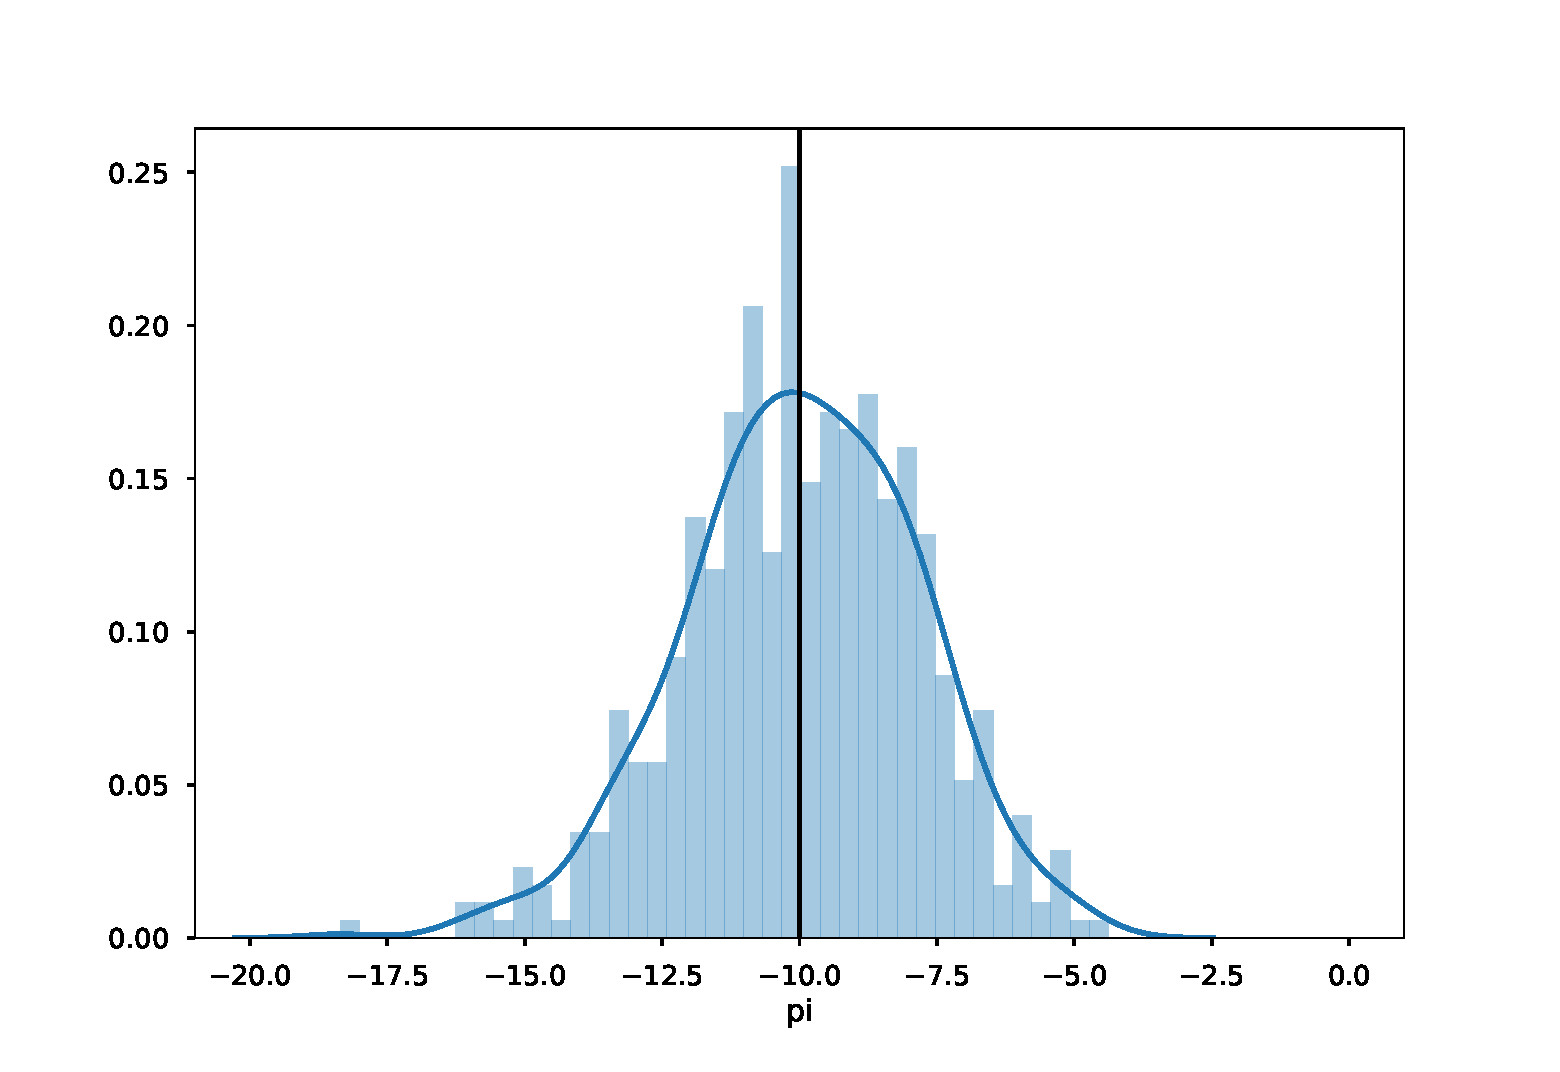
\includegraphics[width=\textwidth, height=\textwidth]{pi_est_500_-0_point_4.pdf}
    \end{subfigure}
    \begin{subfigure}[t]{.32\textwidth}
        \caption[phi = -0.10]{$\phi = -0.10$}
        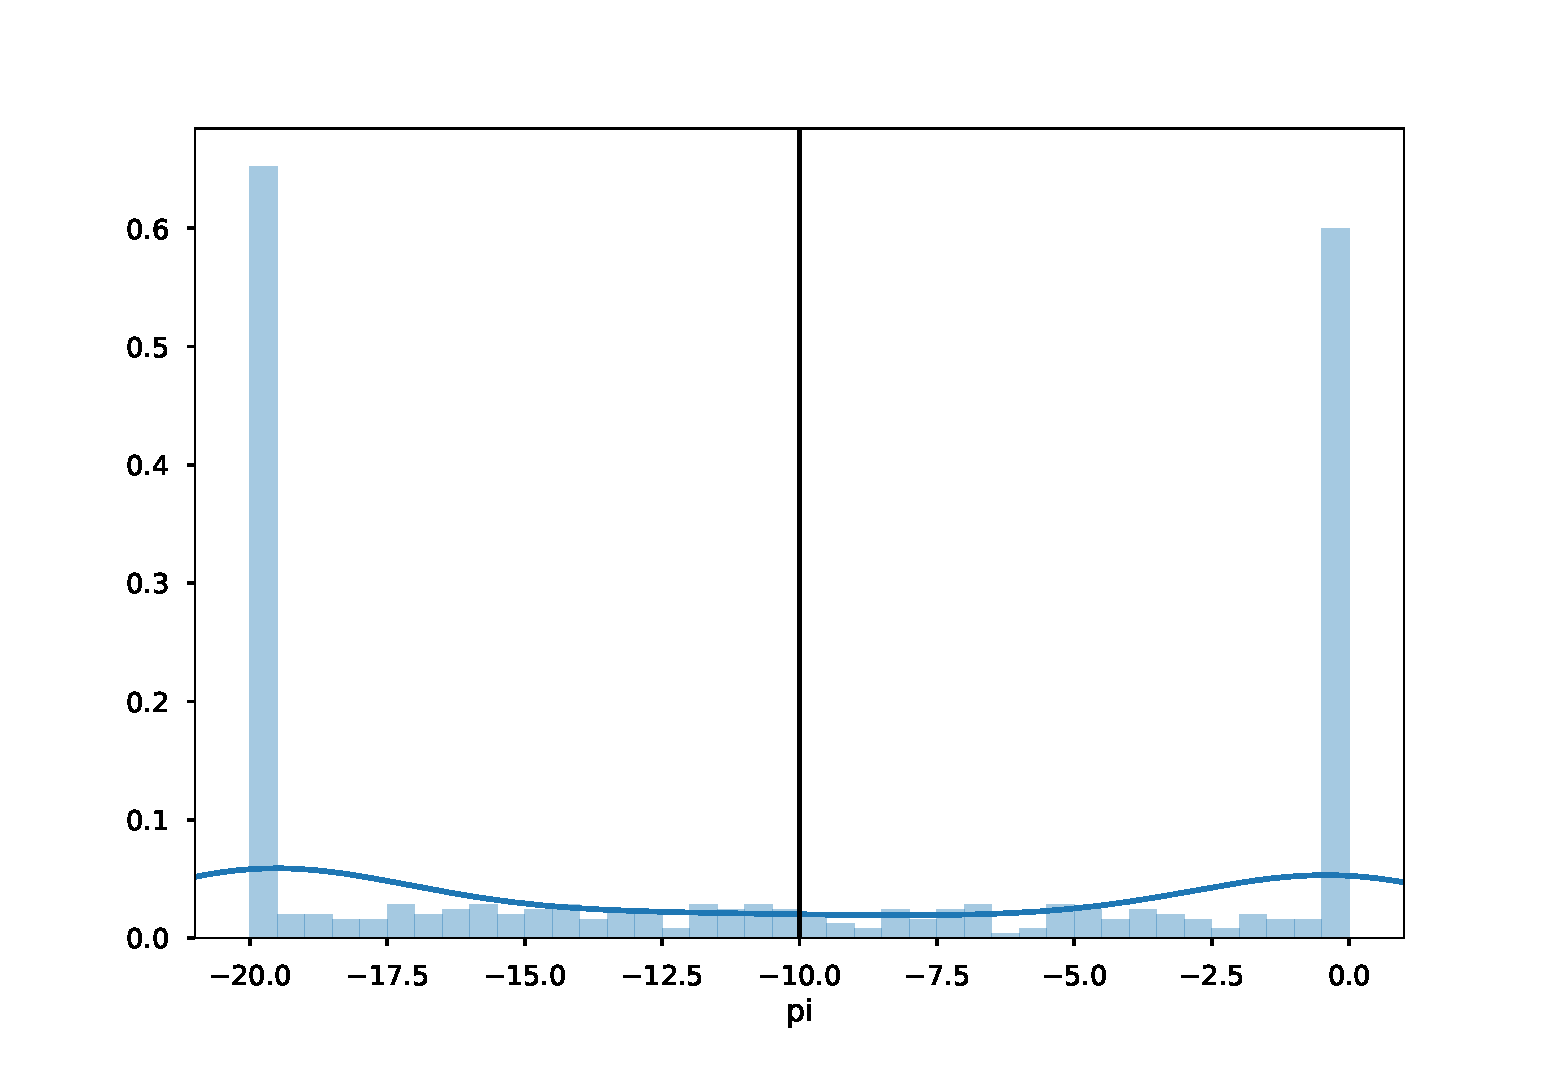
\includegraphics[width=\textwidth, height=\textwidth]{pi_est_500_-0_point_1.pdf}
    \end{subfigure}
    \begin{subfigure}[t]{.32\textwidth}
        \caption[phi = -0.01]{$\phi = -0.01$}
        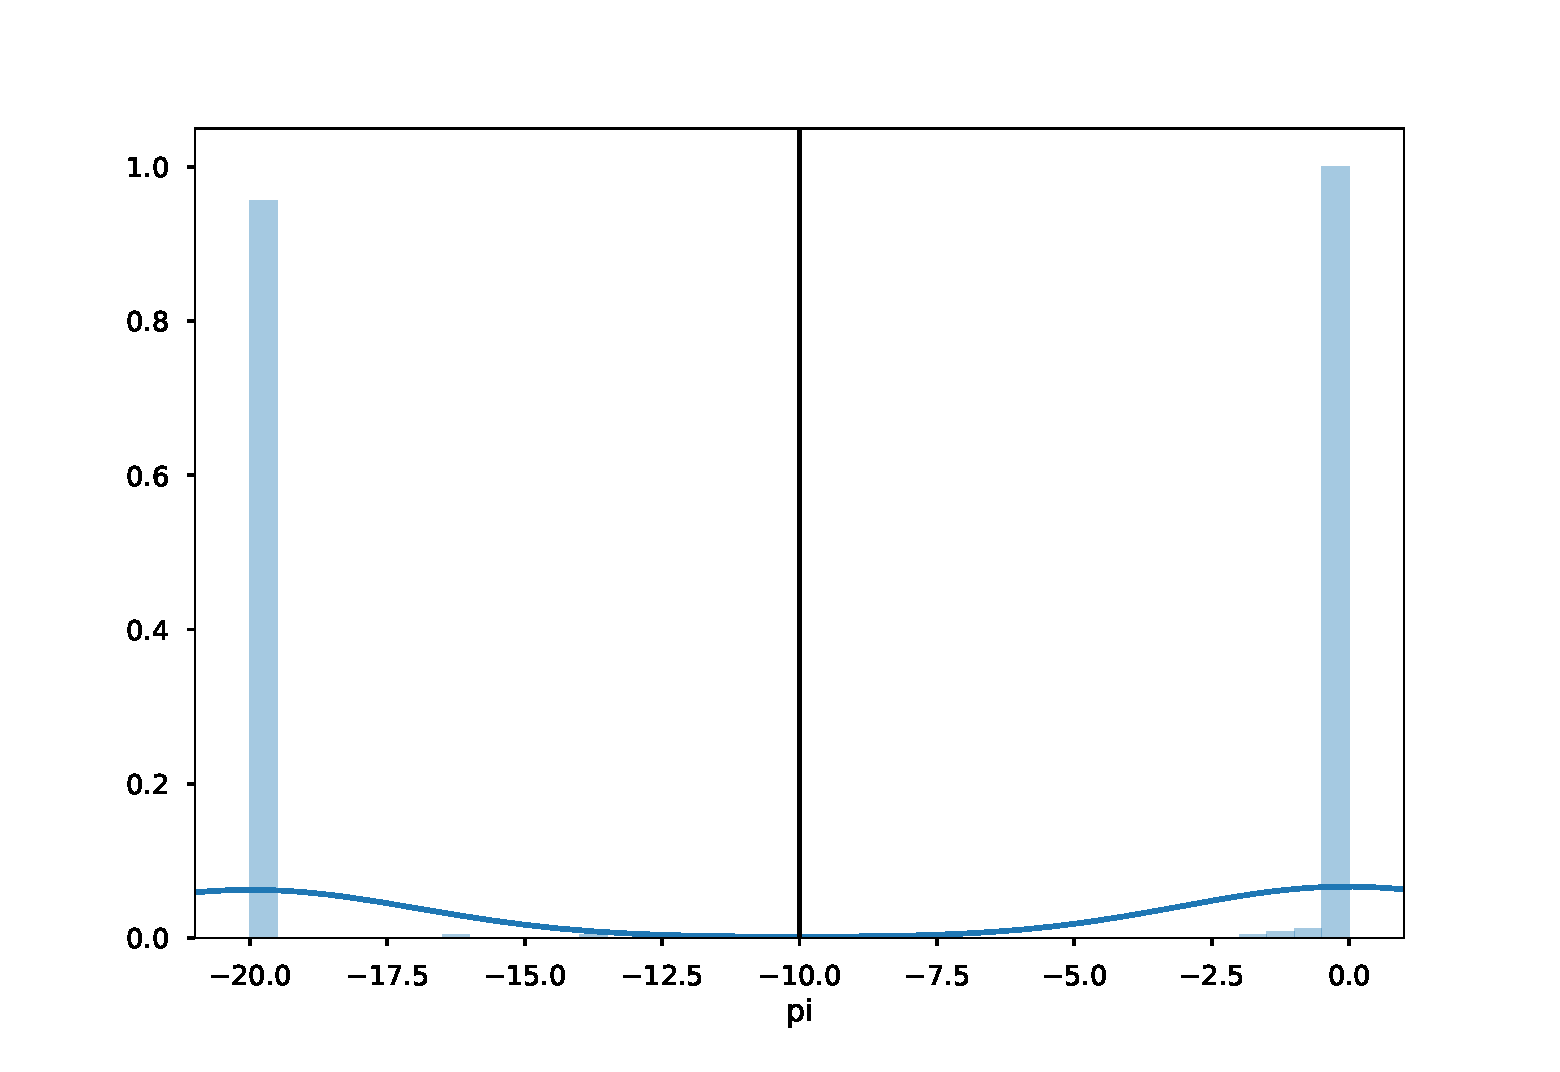
\includegraphics[width=\textwidth, height=\textwidth]{pi_est_500_-0_point_01.pdf}
    \end{subfigure}

\end{figure}

We now report size of the tests in finite-sample using the standard Gaussian Quasi-Likelihood Ratio (QLR) statistic, the Anderson-Rubin (AR) statistic, and the conditional-QLR  proposed here.
Because we have four link functions, the AR-statistic is asymptotically $\chi^2(df=4)$ distributed.
%TODO This is right, isn't it?

\begin{table}[htb]
  
    \centering
    \caption{Finite-Sample Size}
    \label{tbl:test_performance}

  \sisetup{
    round-mode=places,
    round-precision=3,
  }
 
  \begin{tabularx}{\textwidth}{X | *{3}{S} | *{3}{S}}
%
    \toprule
    $\phi$ & {QLR} & {AR} & {CLR}  & {QLR} & {AR} & {CLR} \\
    \midrule
      \multicolumn{7}{c}{Parameter Values used by \textcite{han2018leverage}} \\
    \midrule
    & \multicolumn{3}{c}{$T$ = 37000} & \multicolumn{3}{c}{$T$ = 3700} \\
    \midrule
    -0.01   &           &           &           &       &           &           \\
    -0.10   & 0.03200    & 0.0100    & 0.05400   &       &           &           \\
    -0.40   & 0.0480    & 0.0200    & 0.05000    &       &           &           \\
%
    \midrule
              \multicolumn{7}{c}{Parameters Estimated from the Data} \\
    \midrule
            & \multicolumn{3}{c}{$T$ = 37000} & \multicolumn{3}{c}{$T$ = 3700}  \\
    \midrule
    -0.01   & 0.0600    & 0.0300    & 0.06600                                    \\ 
    -0.10   &           &           &       & 0.084000    & 0.03600 & 0.09000  \\ 
    -0.40   &           &           &       & 0.09200     & 0.06400 & 0.10400  \\
    \bottomrule

  \end{tabularx}

\end{table}

If we look at the upper-right-hand corner of \cref{tbl:test_performance}, we see that the $AR$-statistic is robust, but conservative, as we would expect. We also see that the standard $QLR$-statistic appears to be conservative. The $CLR$ test, on the on the other hand, is robust and has the proper size regardless of the value of $\phi$. The other section in \cref{tbl:test_performance} are less encouraging. Neither the $CLR$ nor the $QLR$ statistic performs well when we use the parameters estimated from the data, even when $\phi = -0.40$. This is likely occurs for two reasons. First,  the variance of $r_{t+1}$ increases with $\phi$, and so $\phi$ is not purely a measure of the signal-to-noise ratio.\footnote{$\Var(r_{t+1}) = 4.5$ when $\phi = -0.01$, and $\Var(r_{t+1}) = 14.7$ when $\phi = -0.04$.} Consequently, the lower right-hand pane of \cref{tbl:test_performance} is not necessarily a good approximation of what happens in the data. Second, even though, $c$ and $\delta$ do not equal zero, the standard errors are large enough that we must truncate their confidence intervals. This likely introduces some non-Gaussianity into the first-stage distribution when $T = 3700$.\footnote{See the discussion around \cref{tbl:reduced_form_parameters} for further discussion.} This causes both the $QLR$ and $CLR$ tests to have improper size even when $\phi$ is large. This is likely also why the $AR$ statistic does not appear to be conservative. The bias induces by the improper first-stage distribution and the inherent conservativeness of that test appear to approximately cancel out in this simulation.  The first-stage distribution in the upper-right-hand, conversely, appears to be well-behaved, and so we do not have similar issues.



\section{Data and Empirical Results}\label{sec:empirics}



\subsection{Data}

The two series we need to estimate the model are $r_{t+1}$ and $\sigma^2_{t+1}$, and $\sigma^2_{t+1}$ must be the volatility of $r_{t+1}$.  That is, we need the appropriately defined variance of $r_{t+1}$ to equal $\sigma^2_{t+1}$ in expectation as discussed in \cref{sec:deriving_conditional_mean}.  Since this condition is automatically satisfied by the integrated volatility and daily return, we use high-frequency data to estimate $\sigma^2_{t+1}$ and use the associated daily return for $r_{t+1}$.  

We need a market index so that the risk prices we estimate are not prices of risk investors face in practice. The do not the asset's risk the asset to be diversifiable. We use SPY, (SPDR S\&P 500 ETF Trust), which is an exchange-traded fund that mimics the S\&P 500.  

We use the procedure \textcite{sangrey2018jumps} develops to estimate the integrated total volatility, which is the instantaneous expectation of the price variance, i.e., the time-derivative of the predictable quadratic variation. This measure reduces to the integrated diffusion volatility if prices have continuous paths. He shows in simulation that his method works well in the presence of market microstructure noise.

Since this paper only use one asset, and SPY is one of the most liquid assets traded, we can essentially choose the frequency at which we want to observe the underlying price. In order to balance market-microstructure noise, computational cost, and efficiency of the resultant estimators we sample at the \SI{1}{\second} frequency. The data starts in 2003 and ends in September 2017. Since the asset is only traded during business hours, this leads to \num{3713} days of data with an average of $\approx \num{24000}$ observations per day.  We compute $r_{t+1}$ as the daily return from the open to close of the market because this is the interval over which the volatility is calculated; hence, we do not need to specify the relationship between overnight and intra-day returns.  

We preprocess the data using the pre-averaging approach as in \textcites{podolskij2009bipower, aitsahalia2012testing}. This procedure is known not to affect the consistency of the estimation procedure. The basic idea is rather simple. We average the price over a small interval to remove the noise. If we pick the rates at which we shrink the interval to appropriately balance averaging away the noise and estimating the instantaneous variation, the estimators will be consistent even in the presence of noise.  

\begin{figure}[htb]

    \centering
    \caption{S\&P 500 Volatility and Log-Return}


    \begin{subfigure}[t]{.54\textwidth}
        \label{fig:spy_dynamics}
        \caption{Time Series}
        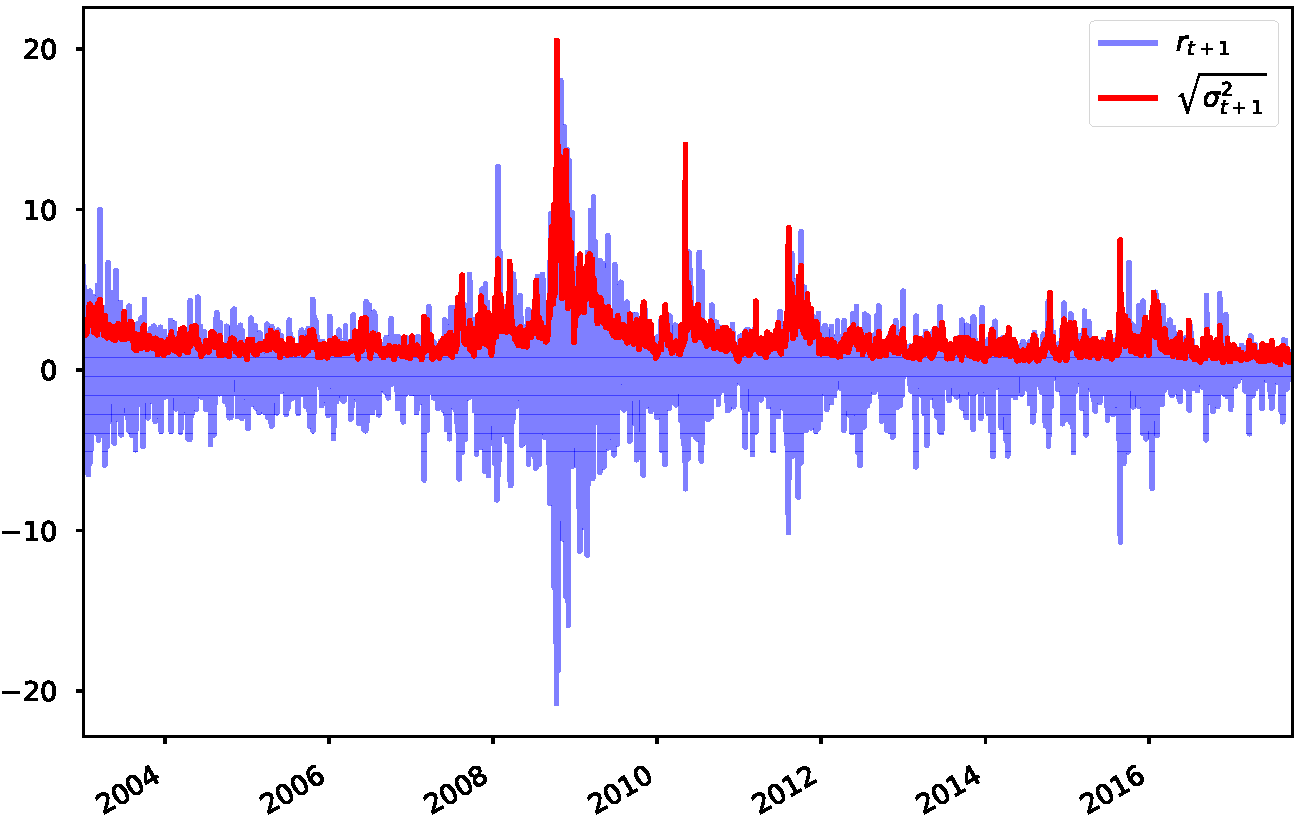
\includegraphics[width=\textwidth, height=.81\textwidth]{time_series.pdf}
    \end{subfigure}%
%
    \hfill
%
    \begin{subfigure}[t]{.44\textwidth}
        \label{fig:spy_static}
        \caption{Joint Distribution}
        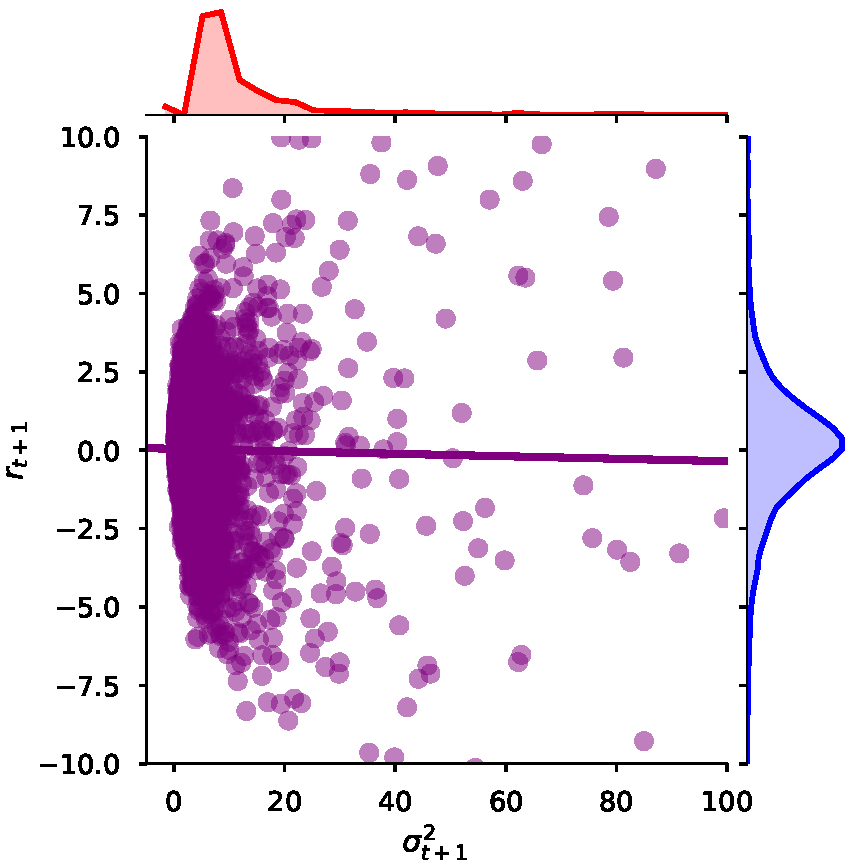
\includegraphics[width=\textwidth, height=\textwidth]{joint_dist.pdf}
    \end{subfigure}
\end{figure}


We also plot the joint unconditional distribution to see the static relationship between the two series are related. The volatility has a long-right tail (it has has the typical gamma-type distribution) and the returns have a bell-shaped distribution. They are also slightly negative related as can be seen by the regression line in the joint plot.

We also report a series of summary statistics.  The volatility and returns are weakly negatively correlated, corroborating the work by \textcites{bandi2012timevarying, aitsahalia2013leverage}.  

\begin{table}[htb]

    \centering
    \caption{Summary Statistics}
    \label{tbl:summary_stats}


    \sisetup{
      table-align-text-pre=false,
      table-align-text-post=false,
      round-mode=places,
      round-precision=2,
      table-space-text-pre=\lbrack,
      table-space-text-post=\rbrack,
    }

    \begin{tabularx}{.5\textwidth}{X | S S}
        \toprule
        & {$r_{t+1}$}  & {$\sigma^2_{t+1}$} \\
        \midrule
            Mean & 0.023421 & 5.621287 \\
            \rowcolor{gray!20}
            Standard Deviation & 2.350165 & 14.458446\\
            Skewness & -0.312 & 12.209 \\
            \rowcolor{gray!20}
            Kurtosis & 10.055 & 240.401 \\
            Correlation & \multicolumn{2}{c}{\num{-0.024379}} \\
        \bottomrule
    \end{tabularx}

\end{table}


\subsection{Estimates}

We now report the reduced-form parameters  estimates and associated confidence intervals.  We only report the reduced-form parameters that true determinant of the model, i.e., they are necessary to simulate the model. The other reduced-form parameters are known function of these parameters and the structural parameters and so have only useful in that the estimation procedure itself. The confidence intervals reported here use the Gaussian limiting theory, ($\pm 1.96$ standard errors)  but we truncate at the edge of the parameter space if necessary. Although, these reduced-form parameters can be estimated directly from the data, disentangling $c$ and $\delta$ is difficult and so the estimation procedure responds appropriately by reporting relatively large standard errors.  


\begin{table}[htb]
    \caption{Reduced-Form Parameter Estimates} 
    \label{tbl:reduced_form_parameters}

    \centering
    \sisetup{
        table-align-text-pre=false,
        table-align-text-post=false,
        round-mode=places,
        table-alignment=center,
    }

    \begin{tabularx}{.5\textwidth}{X | S >{{(}} S[table-space-text-pre={(}] <{{,\,}}
        S[table-space-text-pre={\hspace{-1cm}}] <{{)}}}
%
        \toprule
        & {Point Estimate}  & \multicolumn{2}{c}{Confidence Interval} \\
        \midrule
        $c$         & 3.112013  & 0.00 & 7.379227 \\
        % $c$         & 3.112013  & -1.155201 & 7.379227 \\
        \rowcolor{gray!20}
        $\delta$    & 0.2678579 & 0.00 & 3.007632 \\
        % $\delta$    & 0.2678579 & -2.471916 & 3.007632 \\
        $\rho$      & 0.807506  & 0.402264  & 1.00 \\
        % $\rho$      & 0.807506  & 0.402264  & 1.212748 \\
        \bottomrule 
   \end{tabularx}
\end{table}


We are interested in not just the reduced-form parameters.  We also want estimates for the $\phi$ and the risk prices.  Since $\phi < 0$, our estimator is consistent and do the point estimate is a meaningful number.  We report the \SI{95}{\percent} confidence intervals by taking computing the joint confidence interval above, and then projecting down to the each of the components.


\begin{table}[htb]
    \caption{Structural Parameter Estimates} 
    \label{tbl:structural_param_estimates}

    \centering
    \sisetup{
        table-align-text-pre=false,
        table-align-text-post=false,
        round-mode=places,
        round-precision=2,
        table-alignment=center,
    }

    \begin{tabularx}{.5\textwidth}{X | S >{{(}} S[table-space-text-pre={(}] <{{,\,}}
        S[table-space-text-pre={\hspace{-1cm}}] <{{)}}}
%
        \toprule
        & {Point Estimate}  & \multicolumn{2}{c}{Confidence Interval} \\
        \midrule
        $\phi$      & -0.302417  & 0.30 & -0.20 \\
        \rowcolor{gray!20}
        $\pi$       & -0.115097 & -0.2500 & 0.0 \\
        $\theta$      & 0.516140  & 0.20 & 0.6 \\
        \bottomrule 
   \end{tabularx}
\end{table}

The parameters in \cref{tbl:structural_param_estimates} have a few notable features.  First, we can reject $\phi = 0$ at the \SI{95}{\percent} level.  We cannot, however, reject that $\pi = 0$.  Interestingly, the values for $\phi, \pi$, and $\theta$ reported by \textcite{han2018leverage} lie outside our confidence regions of each of the parameters. They calibrate $\pi = 10$, and then estimate the remaining parameters. Since their calibration of $\pi$ is badly  misspecified, their resulting estimates for $\theta$ is biased in finite sample. To be fair to them, our estimates do not lie outside their confidence intervals. Even though, our estimation procedure for the parameters individually is  conservative, as induced by the projection above, our estimates are still more precise in practice.  This is likely a result of our estimation procedure more effectively using the information about the various parameters jointly, which their partially calibrated model is incapable of doing.

The one main issue with the estimates in \cref{tbl:structural_param_estimates} is that they are conservative because we go from joint inference to sub-vector inference by using a projection based procedure.  Plots of confidence region in three dimensions are not particularly easy to understand, and so we report a joint confidence region for the two equity prices.


\begin{figure}[htb]

    \centering
    \caption{Confidence Set for Risk Prices}
    \label{fig:confidence_region}

    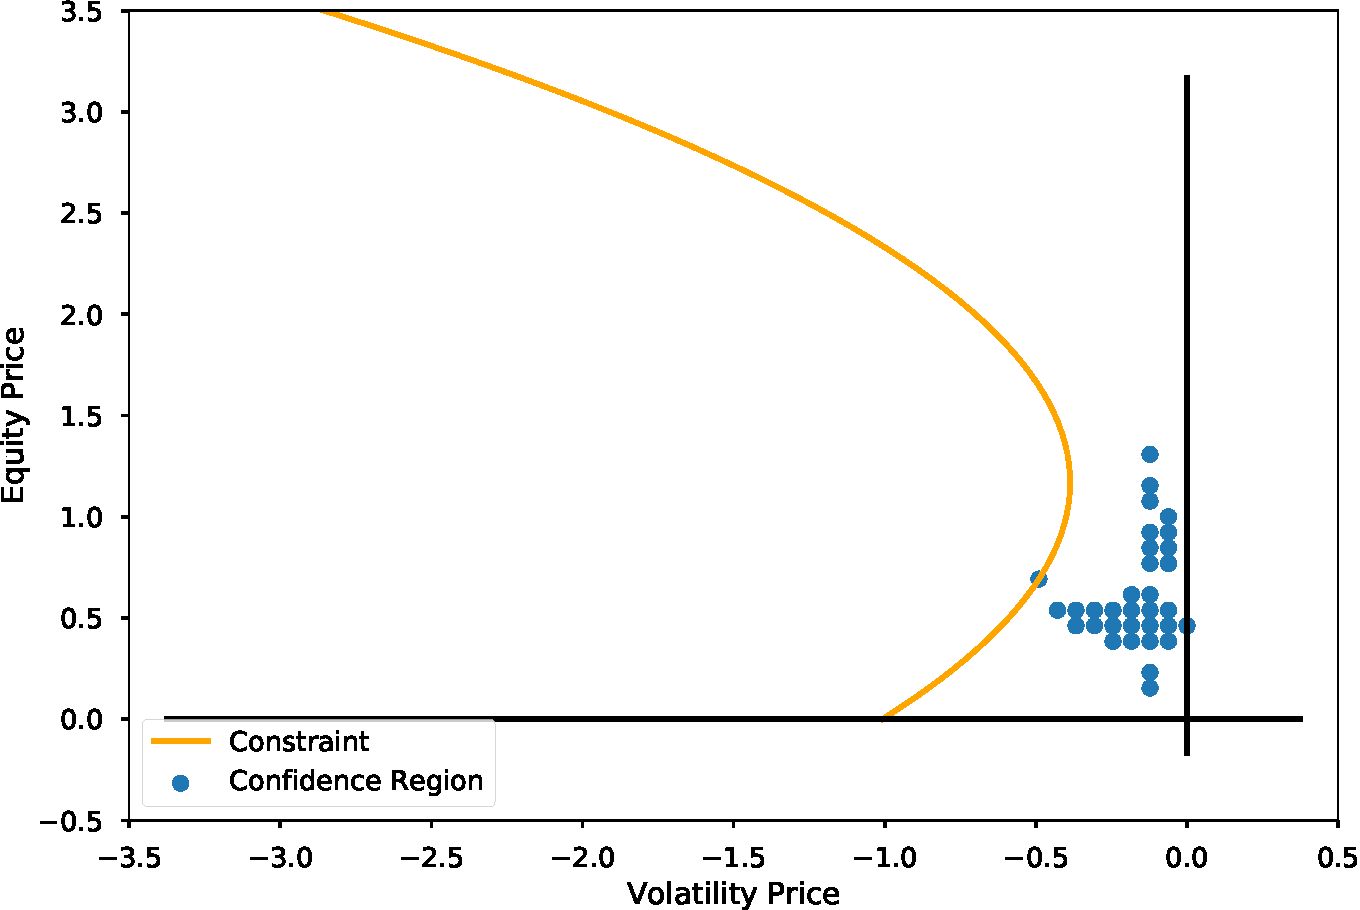
\includegraphics[width=.5\textwidth]{confidence_region.pdf}
\end{figure}

The confidence region is approximately rectangular, and so the projection inference we reported in \cref{tbl:structural_param_estimates} is likely not particular conservative. Furthermore, since we plotted the constraint on the potential value of the parameters, we can see that except for $\pi < 0$, the other constraints do not bind in practice. It is worth noting that there no reason to assume that confidence region has to be connected. The joint likelihood appears to be multi-modal but since the asymptotic distribution is not Gaussian, this not surprising.


\section{Conclusion}

In structural stochastic volatility models such as the one developed here, changes in the volatility affect returns through two channels. First, the investor's willingness to tolerate high volatility in order to get high expected return as measured by the price of market risk. Standard economic models  imply there is a static trade-off between risk and expected return. Consequently, when the risk changes the expected return must change to restore equilibrium. However, investors may also be directly averse to changes in future volatility, and the empirical evidence shows that they are. \Textcite{han2018leverage} shows that we can disentangle these two channels through their differing relationships to the leverage effect. However, estimating the leverage effect is quite difficult, \parencite{aitsahalia2013leverage}. This poses a subtle identification that invalidates standard inference. When the data's signal-to-noise ratio is small, as it is here, standard tests and confidence intervals provide misleading results. We adopt the discrete-time exponentially-affine  of \textcite{han2018leverage} and adapt weak identification methods  to this framework to ensure that the resulting confidence intervals are robust.

In particular, we develop a minimum distance criterion that links the market risk price, the volatility risk price, and the leverage effect to a series of well-behaved reduced-form parameters which govern the return and volatility's joint distribution. We do this by adapting the conditional quasi-likelihood ratio test (CLR) \textcite{andrews2016conditional} develop in a GMM framework to a minimum distance framework. The resulting CLR test is uniformly valid. We invert this test to derive a robust confidence set. We then apply this methodology to data on the S\&P 500 and show that the market risk price lies in $(0.20, 0.60)$ yearly percentage points, and the volatility risk price lies in $(-0.20, 0.00)$. These estimates are both substantially smaller in magnitude than the values chosen by  \textcite{han2018leverage}.


\clearpage


\phantomsection
\addcontentsline{toc}{section}{References}
\printbibliography
\clearpage

\begin{appendices}


\section{Model Characterization}\label{app:model_characterization}

\begin{lemma}[Linearity of $\beta$ and $\gamma$]
 \label{lemma:linearity_of_physical_functions}
 Letting $\sigma^2_{t+1}$ be the integrated volatility of a process with return $r_{t+1}$.  Assume that $\sigma^2_{t+1}$ and $r_{t+1}$ follow a bivariate CAR(1) process parametrized as in \cref{defn:physical_vol_dynamics} and \cref{defn:physical_return_dynamics}.  Then $\beta''(0)$ and $\gamma''(0)$ both equal zero.
\end{lemma}

\begin{proof}
 By the \Ito\ Isometry, and the definition of $r_{t+1}$ as an integrated variance, the following holds for the returns' predictable information set $\F^r_{t-}$. 

 \begin{equation}
  \Var\left(r_{\tau+1}\mvert \F_{\tau-}\right) \leq \E\left(r^2_{\tau+1} \mvert \F_{\tau-}\right) 
  = \E\left(\sigma^2_{t+1}\mvert \F_{\tau-}\right)
 \end{equation}

 The integrated volatility is predictable, and so $\sigma^2_{t+1}$ is contained in the return's predictable $\sigma$-algebra. 

 Consequently, $\Var\left(r_{t+1} \mvert \sigma^2_t, \sigma^2_{t+1}\right) \leq \sigma^2_{t+1}$ In addition, variance must always be positive, and so $\Var\left(r_{t+1} \mvert \sigma^2_t, \sigma^2_{t+1}\right) \geq 0$.

 Since the second derivative of the log-cumulant function evaluated at zero equals the variance, we have the following set of inequalities.

 \begin{gather}
  0 \leq (1 - \phi^2) \sigma^2_{t+1} - \beta''(0) \sigma^2_t - \gamma''(0) \leq
  \sigma^2_{t+1} 
%
  \intertext{Dividing through by $\sigma^2_{t+1}$ and pulling the first term outside}
%
  \label{eqn:second_derivative_inequalities}
  \implies \phi^2 - 1 \leq -\frac{1}{\sigma^2_{t+1}} \left(\beta''(0) \sigma^2_t +
  \gamma''(0)\right) \leq \phi^2 
%
 \end{gather}

 On the outside of the two inequalities we have constants, and the distribution of $\sigma^2_{t+1}$ given $\sigma^2_t$ is not bounded away from zero.  Consequently, the only way for \cref{eqn:second_derivative_inequalities} to hold for all $\sigma^2_{t+1}$ is if the term inside the parentheses equals zero.

 \begin{equation}
  0 = \beta''(0) \sigma^2_t + \gamma''(0)
 \end{equation}

 However, the only way for this to hold is for both $\gamma''(0)$ and $\beta''(0)$ to equal zero.
 This plus the conditional Gaussianity of the returns implied by the parametric model implies that $\gamma$
 and $\beta$ are both linear.

\end{proof}


\sdfConstants*

\begin{proof}

\begin{equation}
 \label{eqn:reweigted_sdf}
 \E\left[\exp\left(m_0(\theta, \pi) + m_1(\theta, \pi) \sigma^2_t - \pi \sigma^2_{t+1} - \theta r_{t+1}
 \right) \mvert \F_t \right] = 1 
\end{equation}

We can use \cref{eqn:reweigted_sdf} to relate $m_0(\theta, \pi)$ and $m_1(\theta, \pi)$ to the physical measure
functions. 

\begin{gather}
 \E\left[\exp\left(m_0(\theta, \pi) + m_1(\theta, \pi) \sigma^2_t - \pi \sigma^2_{t+1} - \theta r_{t+1}
 \right) \mvert \F_t \right] = 1 \\
%
 \intertext{By the law of iterated expectations.}
%
 \E\left[ \E\left[\exp\left(m_0(\theta, \pi) + m_1(\theta, \pi) \sigma^2_t - \pi \sigma^2_{t+1}\right)
  \exp\left( - \theta r_{t+1}\right) \mvert \F_t, \sigma^2_{t+1} \right]\right] = 1 \\
%
 \intertext{The second term is the Laplace transform of $r_{t+1}$.}
%
 \E\left[\exp\left(m_0(\theta, \pi) + m_1(\theta, \pi) \sigma^2_t - \pi \sigma^2_{t+1} \right)
  \exp(-C(\theta) \sigma^2_{t+1} - D(\theta) \sigma^2_{t} - E(\theta_2) \mvert \F_t \right] = 1 \\
%
 \intertext{Reorganizing terms.}
%
 \E\left[\exp\left(m_0(\theta, \pi) + m_1(\theta, \pi) \sigma^2_t - D(\theta) \sigma^2_{t} - E(\theta_2)
 \right) \exp(-\left(\pi + C(\theta)\right) \sigma^2_{t+1}) \mvert \F_t \right] = 1 \\ 
%
 \intertext{Substituting in the Laplace transform for $\sigma^2_{t+1}$.} 
%
 \label{eqn:expected_sdf_wrt_PP}
 \E\left[\exp(m_0(\theta, \pi) + m_1(\theta, \pi) \sigma^2_t - D(\theta) \sigma^2_{t} - E(\theta_2) - A(\pi +
 C(\theta)) - B(\pi + C(\theta)) \mvert \F_t \right] = 1 
\end{gather}

\end{proof}

\leverageVersusMeasureChange*


\begin{proof}

 We start by considering the expectation of $\widetilde{r}_{t+1}$ and show that it equals zero.

 \begin{align}
  \E\left[\widetilde{r}_{t+1} \mvert \sigma^2_{t} \right] &= \E\left[\E\left[r_{t+1} - \frac{1 - \phi^2}{2}
  \sigma^2_{t+1} + (1 - \phi^2) \theta \sigma^2_{t+1}\mvert \sigma^2_{t}, \sigma^2_{t+1} \right] \mvert
  \sigma^2_t\right] \\
%
  \intertext{By the conditional Gaussianity of $r_{t+1}$, we can absorb the convexity correction into an
  exponential. Normally, it would introduce a $1/2$ variance term, but that cancels. The second term is a
  measurable with respect to the conditioning information and so is not affected.}
%
  &= \E\left[\log \E\left[\exp(r_{t+1}) \exp((1 - \phi^2) \theta \sigma^2_{t+1})\mvert \sigma^2_{t},
   \sigma^2_{t+1} \right] \mvert \sigma^2_t\right] \\
%
  \intertext{We note that normally, the covariance term would cause the mean to fall, but again that term
  cancels with the second term. We can divide through by $\exp(r_t)$ and $m_{t-1,t}$ because they are
  measurable with respect to $\F_t$, and the remainder of the SDF is also contained within the information
  set, and so we can add it as well (\cref{eqn:log_sdf}).} 
%
  &\propto \E\left[\log \E\left[\frac{\exp(r_{t+1})}{\exp(r_t)} \frac{M_{t,t+1}}{M_{t-1,t}} \mvert
   \sigma^2_t, \sigma^2_{t+1} \right] \mvert \sigma^2_t \right]
%
  \intertext{We can pull the log outside of the outer expectation while adding at most a
  $\sigma^2_t$-measurable term.}
%
  &\propto \log \E\left[\frac{\exp(r_{t+1})}{\exp(r_t)} \frac{M_{t,t+1}}{M_{t-1,t}} \mvert \sigma^2_t
   \right]
%
  \intertext{This is the log expectation of a price change in the price discounted by the change in the
  SDF.}
%
  &= 0
 \end{align}

Because the mean of $\tilde{r}_{t+1}$ given $\sigma^2_t$ does not change in expectation when we condition on
$\sigma^2_{t+1}$ we can apply the \Ito\ Isometry.

\begin{equation}
 \label{eqn:return_var_versus_expected_vol_pp}
 \E\left[\Var\left(\tilde{r}_{t+1} \mvert \sigma^2_t\right) \right] = \E[ \sigma^2_{t+1}]
\end{equation}

Intuitively, volatilities are squared returns, and so they are variances.
The tricky part here is that variances are centered second moments, not the second moments themselves.
The volatilities are also centered second moments, but the centering is not the same in general.
In continuous time, they would only differ by a drift term, which can be ignored, which is why the Ito\ Isometry
usually is used in that context.
Using discrete-time return, as we do here, we first have to appropriately recenter the variables, which is why it
applies to $\widetilde{r}_{t+1}$ but not to $r_{t+1}$.

\end{proof}


\section{Identification Proofs}


\identifiedSet*

\begin{proof}
 Since $Q_{T}$ is a quadratic in terms of deviations between sample and population moment conditions as long as
 the population moment can be inverted to solve for the parameters, the $Q_T$ process identifies them as well. 
 In addition, since we have a sufficient number of exogenous valid instruments the conditioning implied by
 projecting on the instruments does not affect the arguments above. 

 Identifying the four parameters that govern the volatility dynamics is not particularly complicated. 
 We have four parameters and four non-redundant moment conditions.
 The first two equations in \cref{defn:equilibrium_moment_conditions} identify $\rho$ and $c \delta$.
 \cref{eqn:cond_vol_var} identifies $\rho c$ and $c^2 \delta$. 
 This allows us to separately identify $c$ and $\delta$.
 
 Identifying $\phi$ is also relatively straightforward. Since $r_{t+1}$ and $\sigma^2_{t+1}$ are known, as long
 as we know the conditional mean of $r_{t+1}$, then identifying $\phi$ is identified by \cref{eqn:cond_rtn_var}.
 Identifying the conditional mean of $r_{t+1}$ is straightforward because we observe volatility and the
 conditional mean is a linear equation in these variables. 
 

 Identifying the risk prices $\pi$ and $\theta$ is more complicated.
 We have to identify both parameters off of \cref{eqn:cond_expected_rtn_moment}. 
 This is in principle possible because we now have two non-redundant sources of variation in the data ---
 $\sigma^2_t$ and $\sigma^2_{t+1}$.

 The only place that \cref{defn:equilibrium_moment_conditions} that the risk-prices occurs in
 \cref{eqn:cond_expected_rtn_moment}. 
 We showed that $\gamma, \beta$ and $\psi$ functions are independent of $\pi$ if $\phi = 0$ in the discussion
 leading up \cref{eqn:alpha_difference}.
 We further showed that they are not independent if $\phi \neq 0$.
 In addition the dependence of the identification in terms of the non-singularity of the derivatives
 equilibrium conditions in terms of $\pi$ and $\theta$ depends smoothly on $\phi$. 
 This will be important later.
 
\end{proof}



\end{appendices}


\end{document}


